\section{Event Yield in event Pre-selection and Signal Regions}
\label{sec:eventYieldSR}

The background estimation described in Section~\ref{sec:backgrounds_estimation}
and the data are passed through the three-lepton selections described in Section~\ref{sec:eventSelection}.


\subsection{Event Pre-selection}

The three lepton event pre-selection region is used as a starting point for all three signal regions
and follows the selection described in Section~\ref{sec:preselection}. Kinematic distributions
in this region are shown in Figure~\ref{fig:preselection} while the yields are shown 
binned by the lepton flavor combinations in Table~\ref{tab:preselection}. The yields in the individual
signal channels just after pre-selection are shown in Figure~\ref{fig:preselection_nsfos} with systematic uncertainties.
In general, good agreement is observed.
%preselection
\begin{figure}[ht!]
\centering
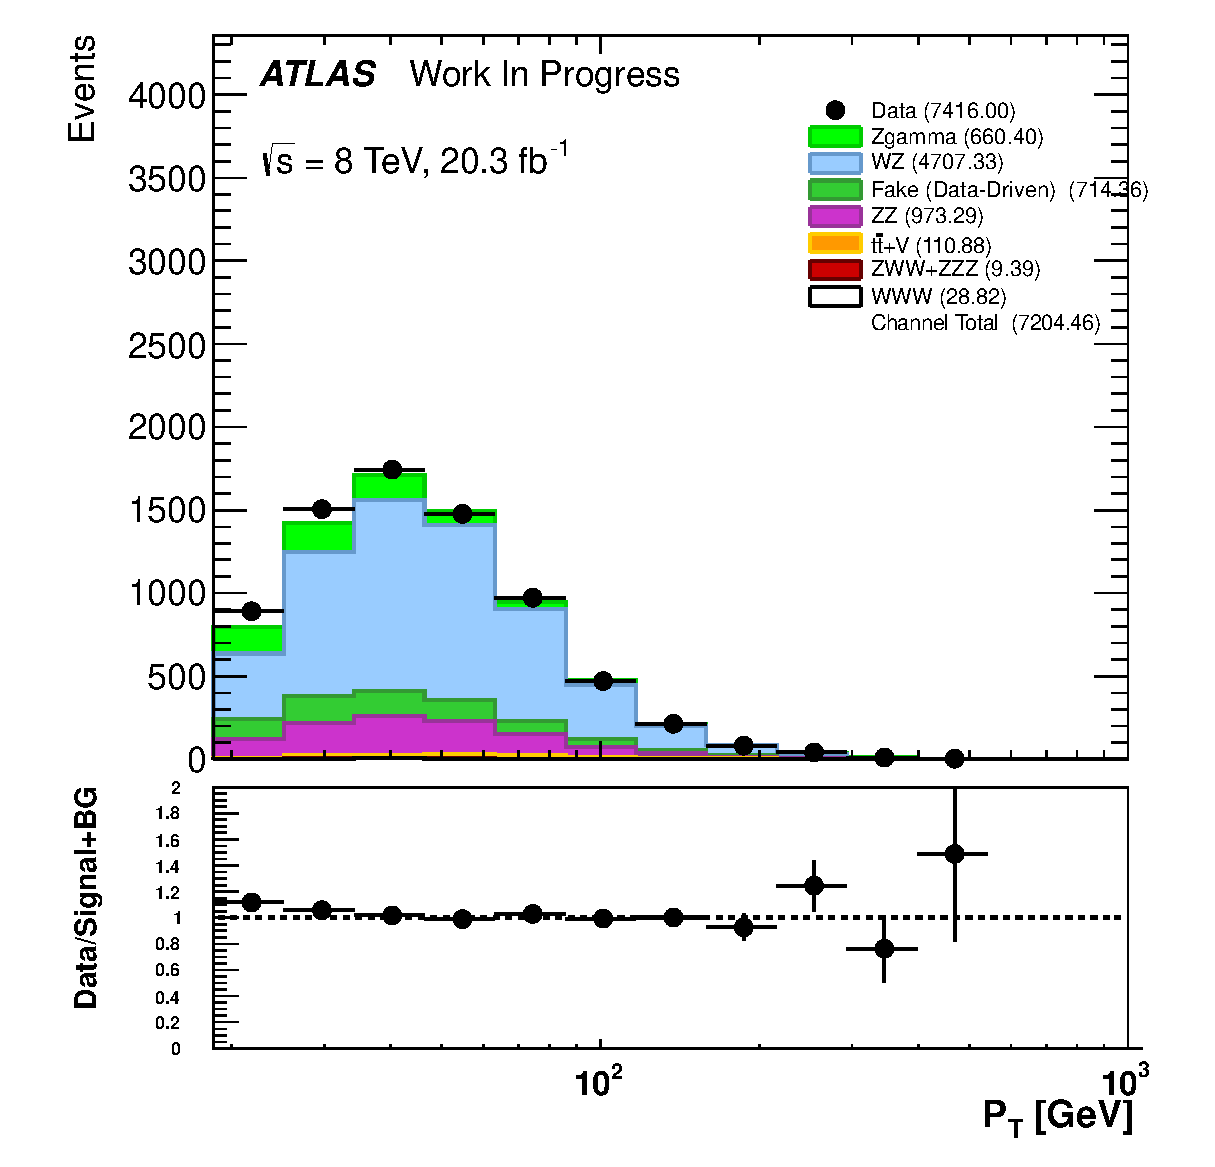
\includegraphics[width=0.3\columnwidth]{figures/preselection/AllLeptonPt_histratio.eps}
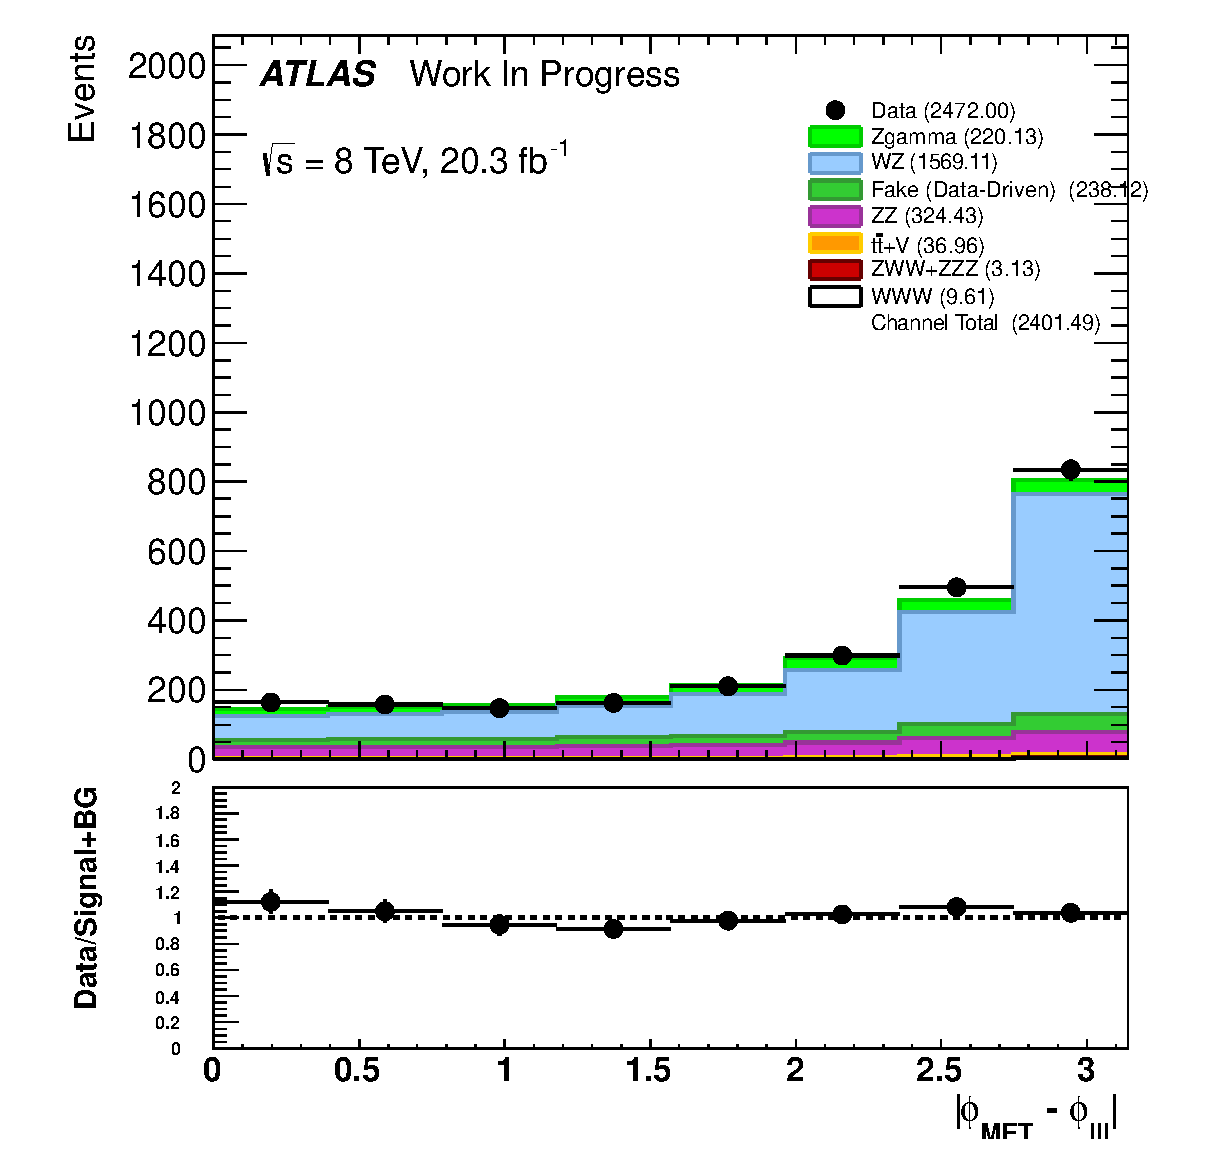
\includegraphics[width=0.3\columnwidth]{figures/preselection/DeltaPhiMET123_Abs_histratio.eps}
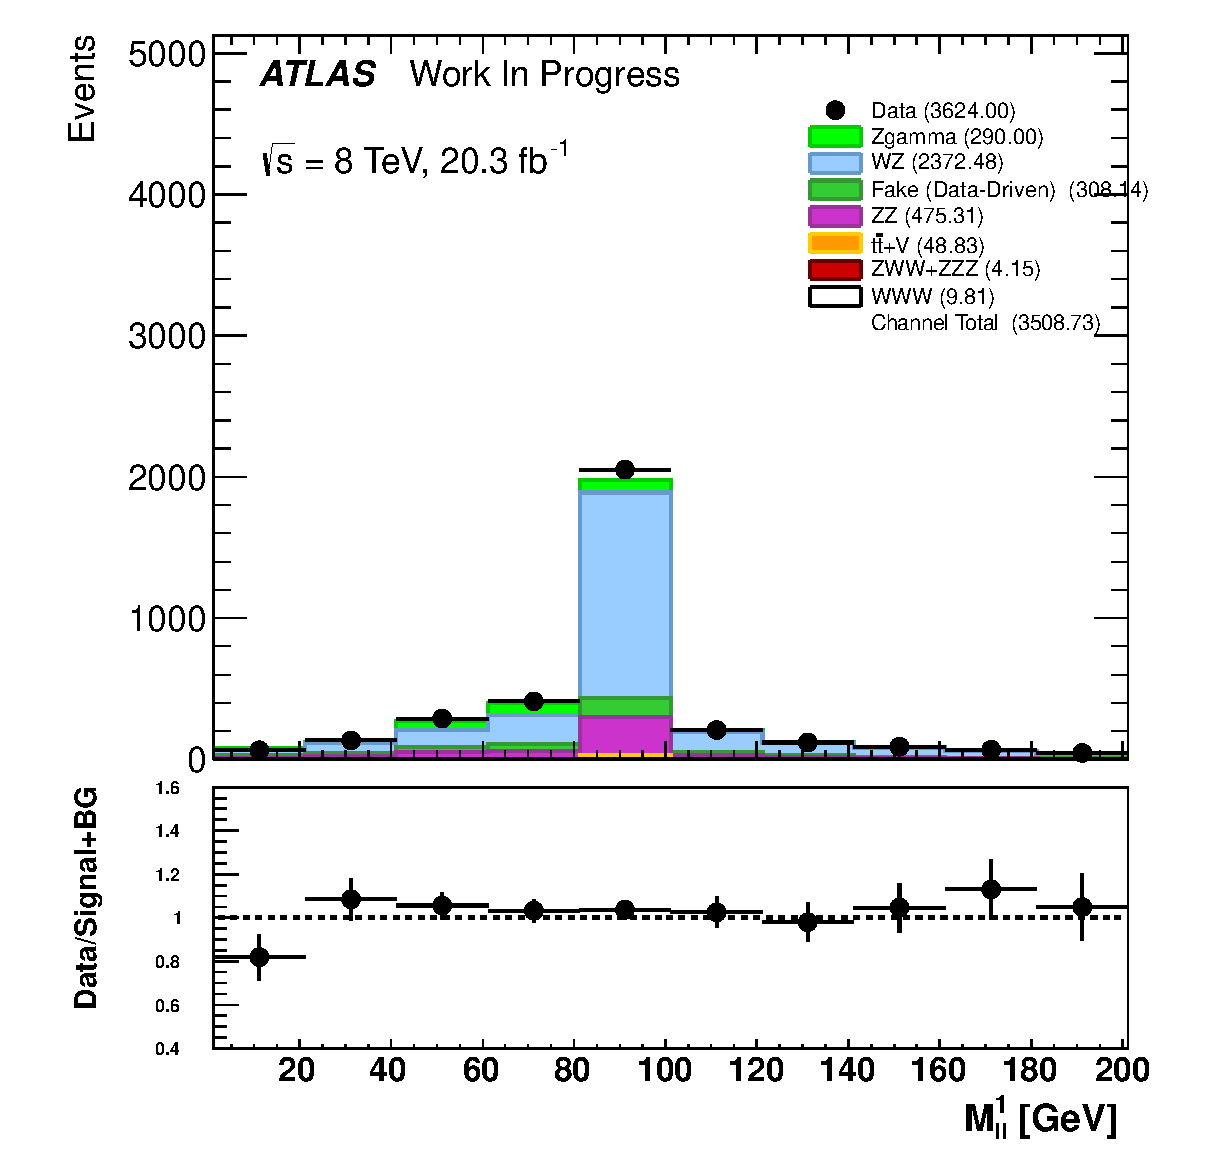
\includegraphics[width=0.3\columnwidth]{figures/preselection/InvariantMassSFOS_histratio.eps}
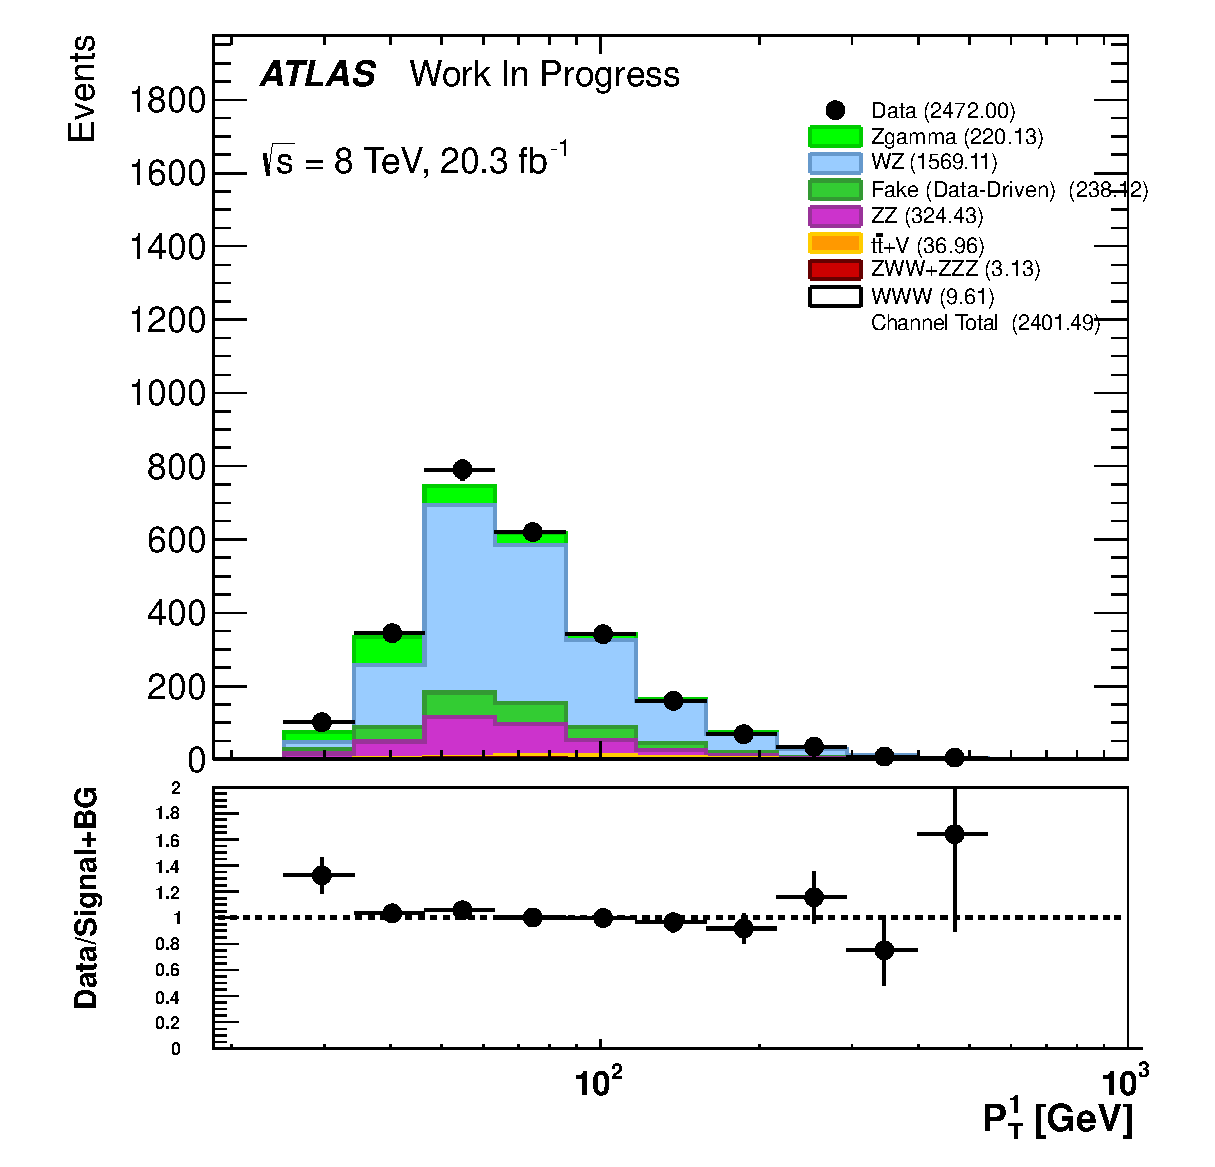
\includegraphics[width=0.3\columnwidth]{figures/preselection/LeadingLeptonPt_histratio.eps}
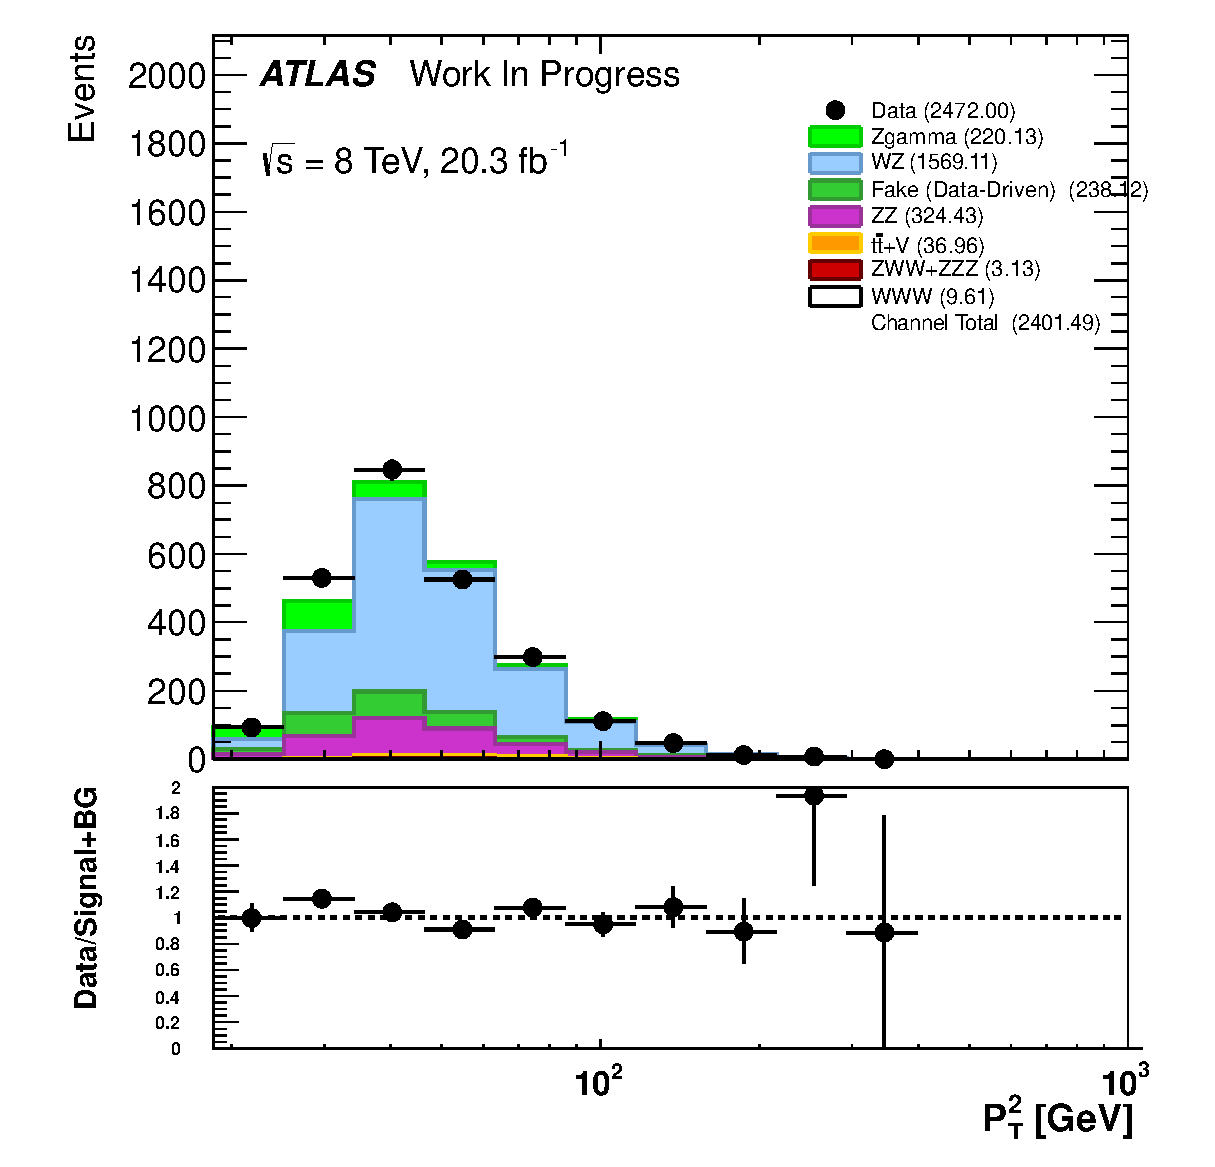
\includegraphics[width=0.3\columnwidth]{figures/preselection/SubleadingLeptonPt_histratio.eps}
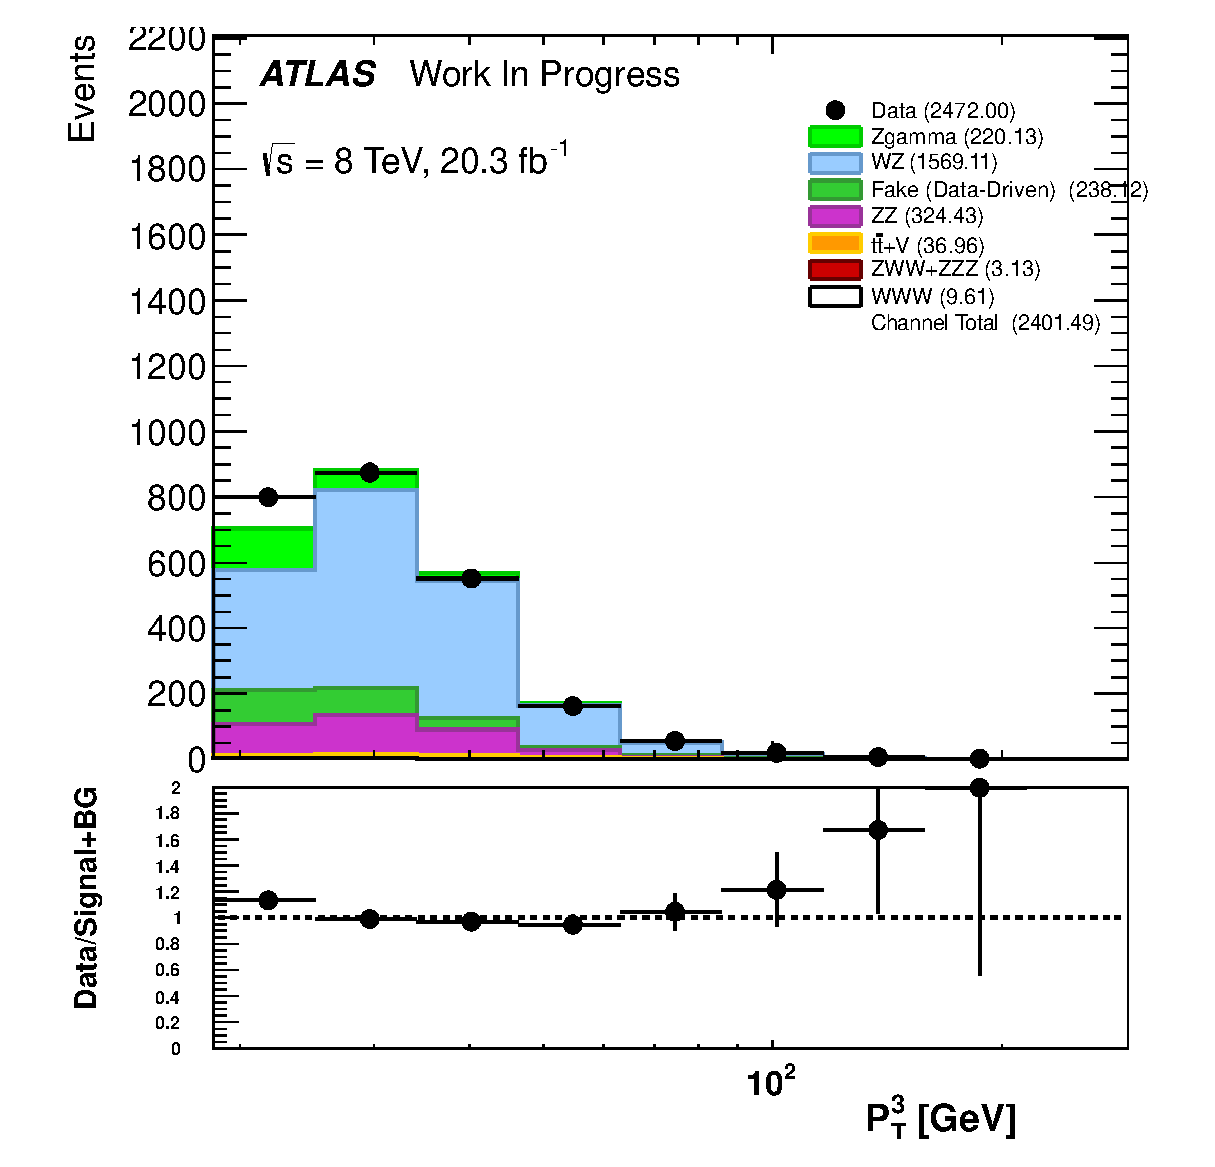
\includegraphics[width=0.3\columnwidth]{figures/preselection/MinimumLeptonPt_histratio.eps}
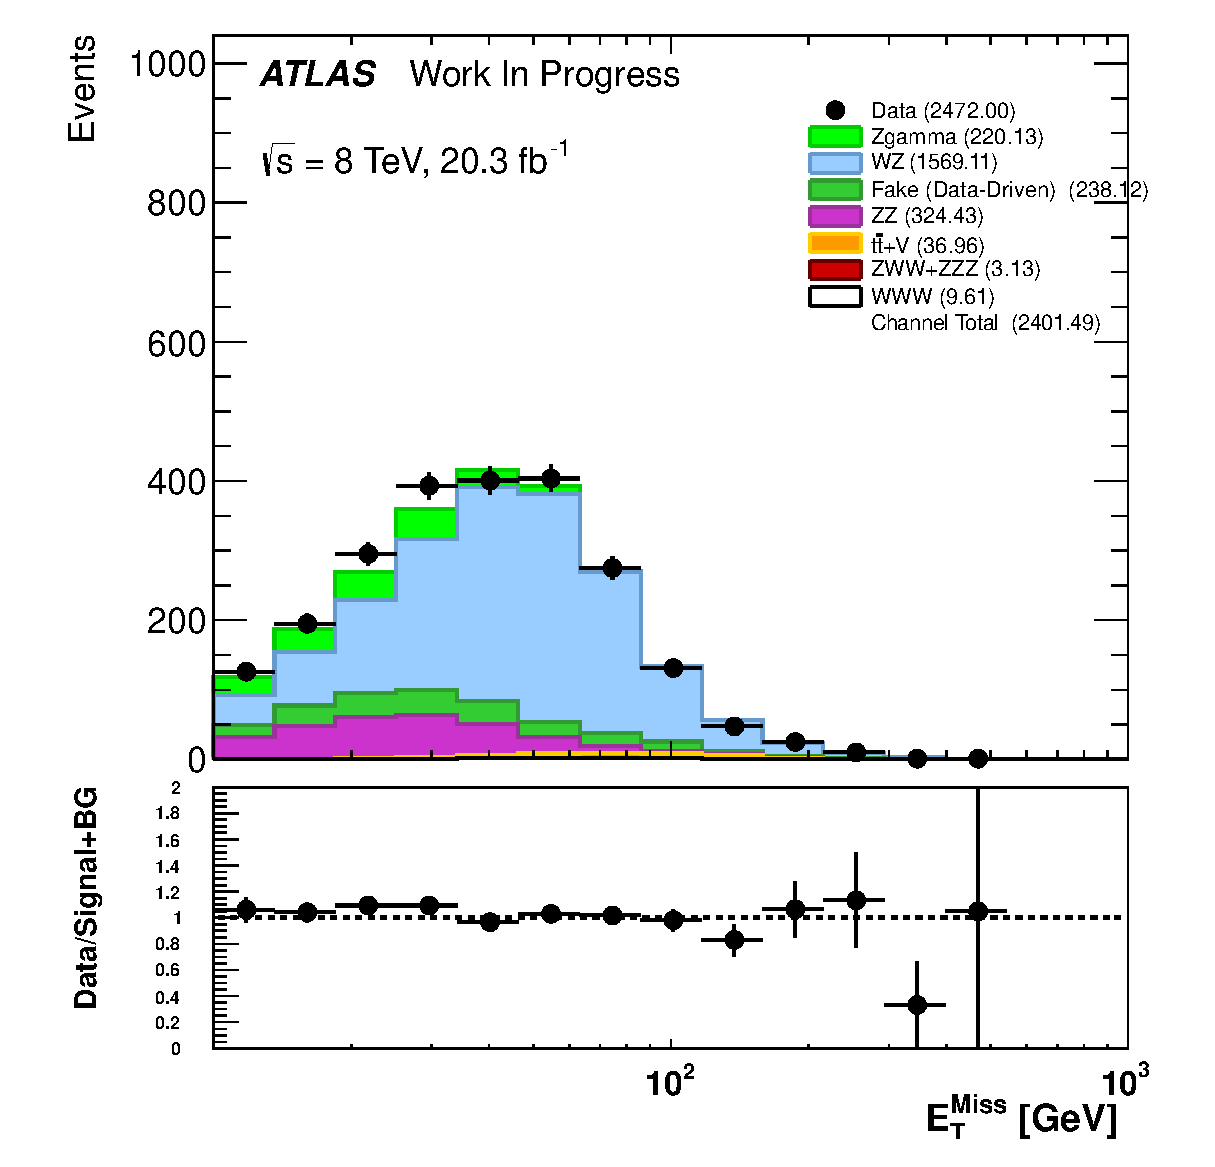
\includegraphics[width=0.3\columnwidth]{figures/preselection/MET_Et_histratio.eps}
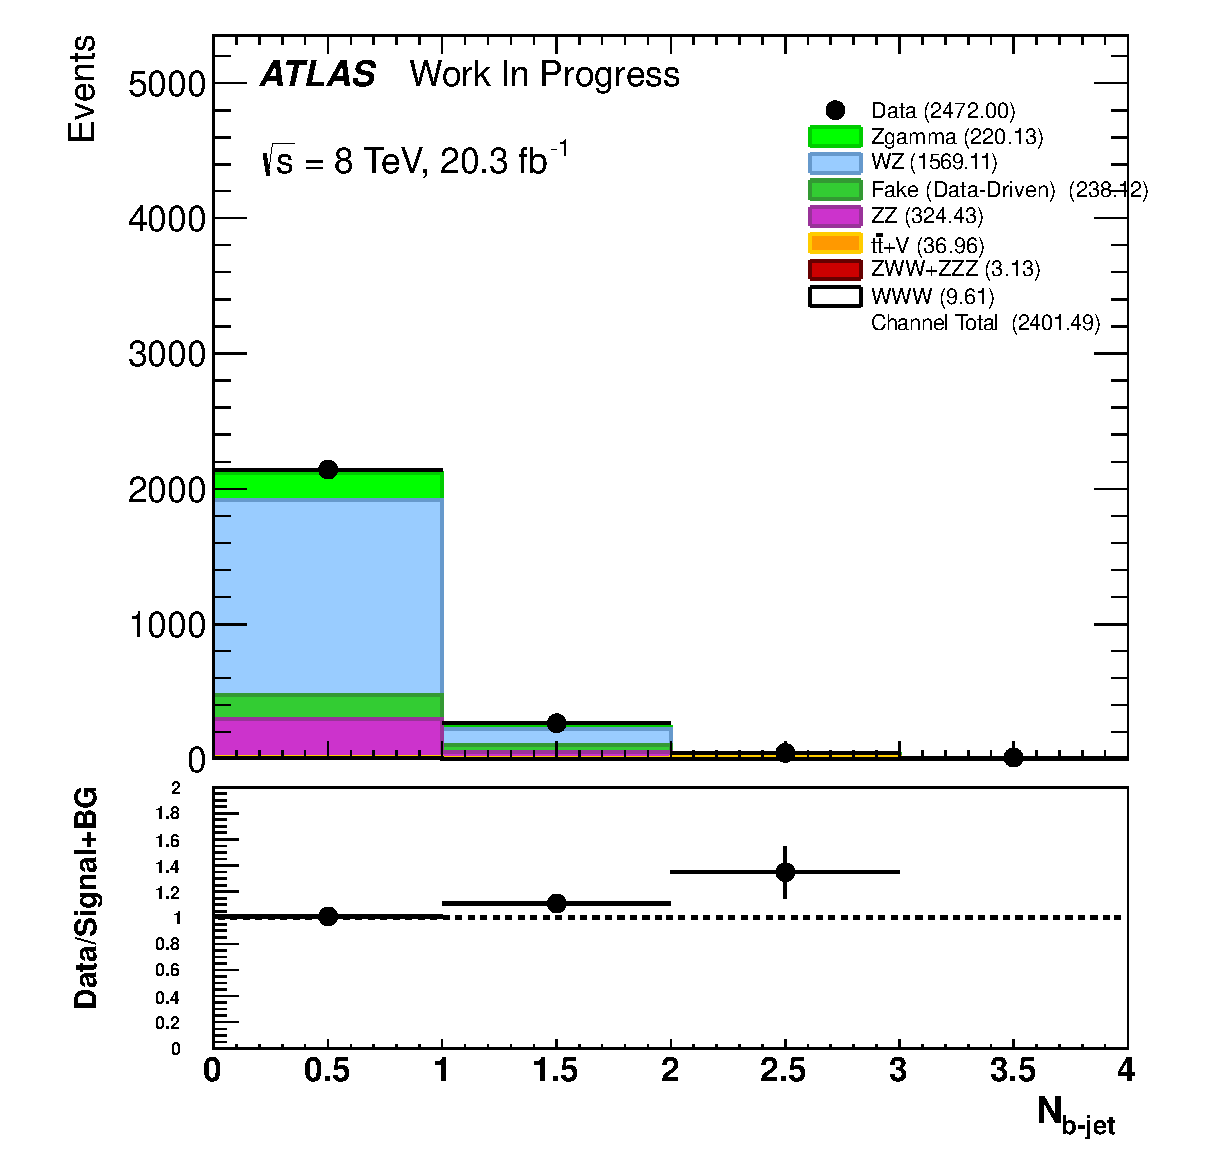
\includegraphics[width=0.3\columnwidth]{figures/preselection/NBTaggedJets_histratio.eps}
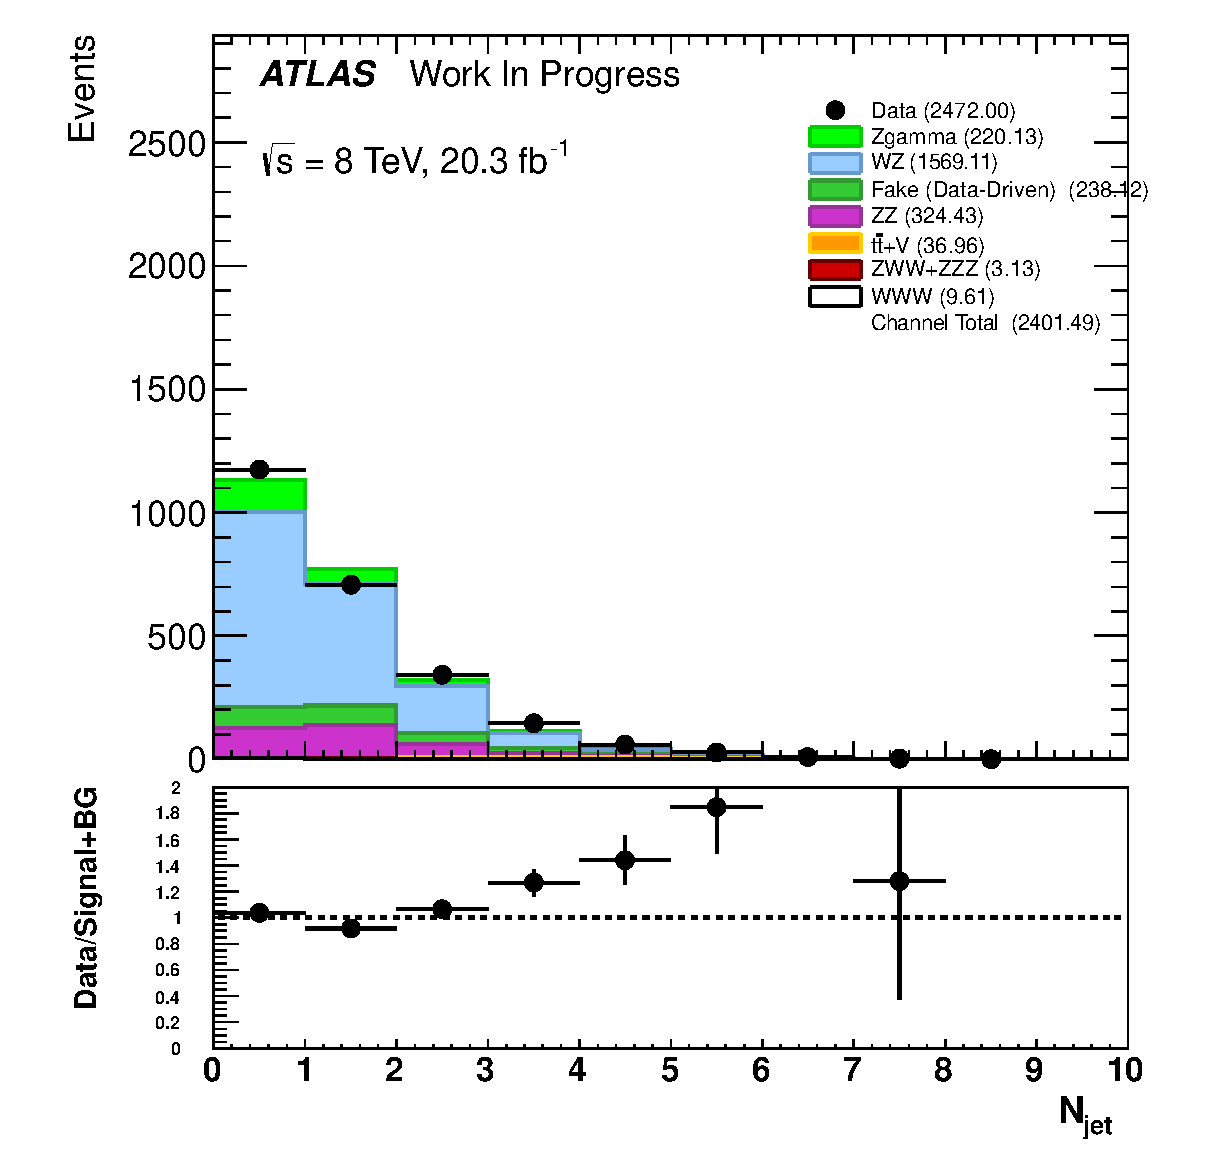
\includegraphics[width=0.3\columnwidth]{figures/preselection/NJets_histratio.eps}
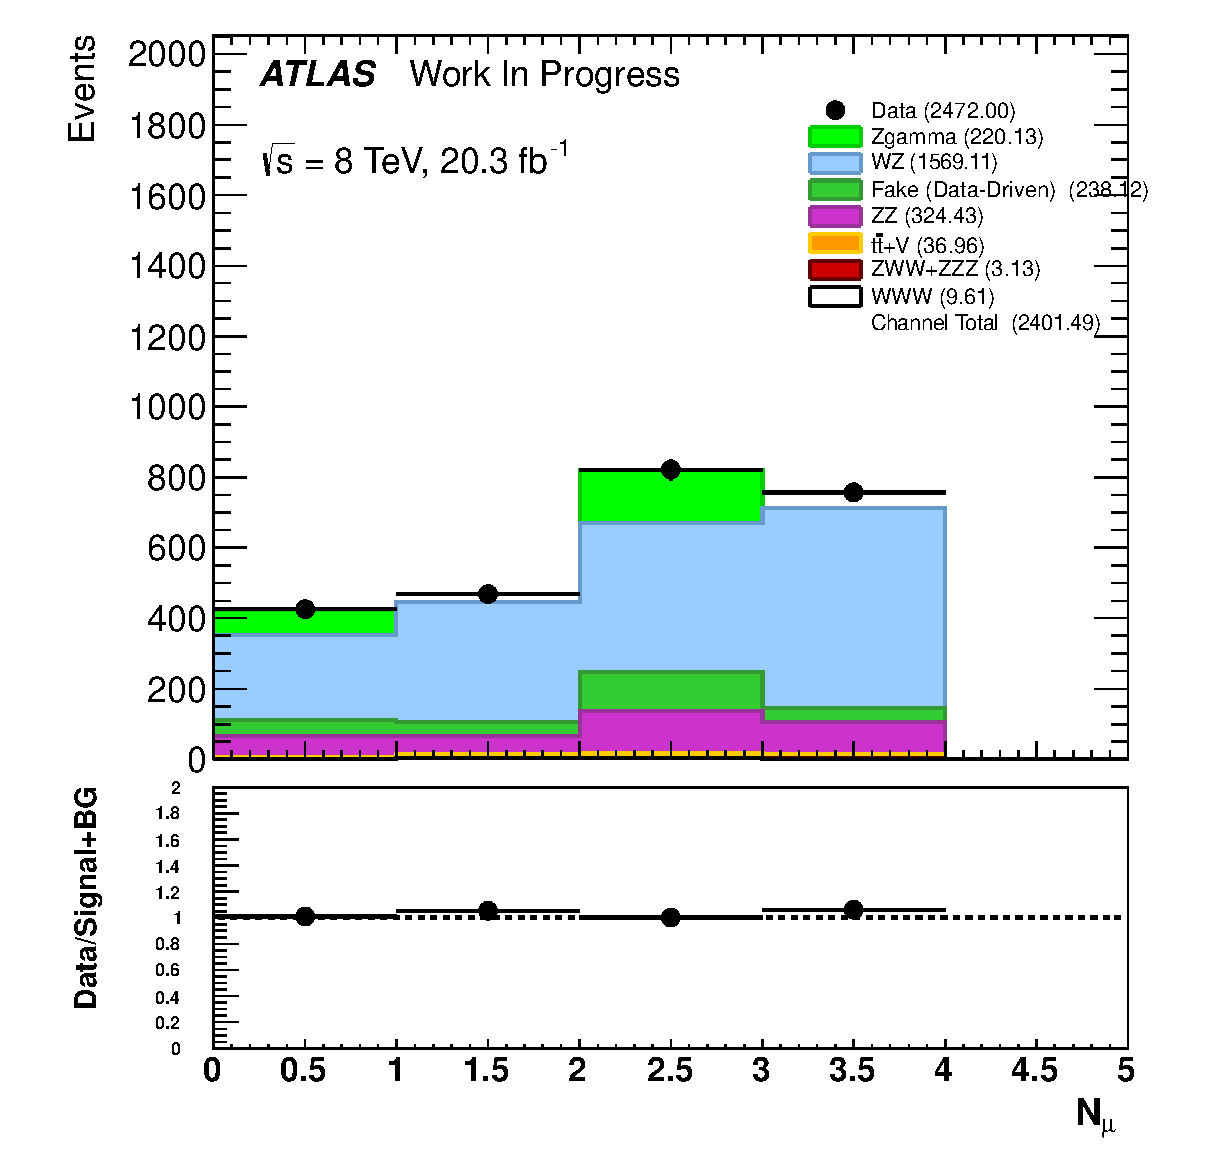
\includegraphics[width=0.3\columnwidth]{figures/preselection/NMuons_histratio.eps}
%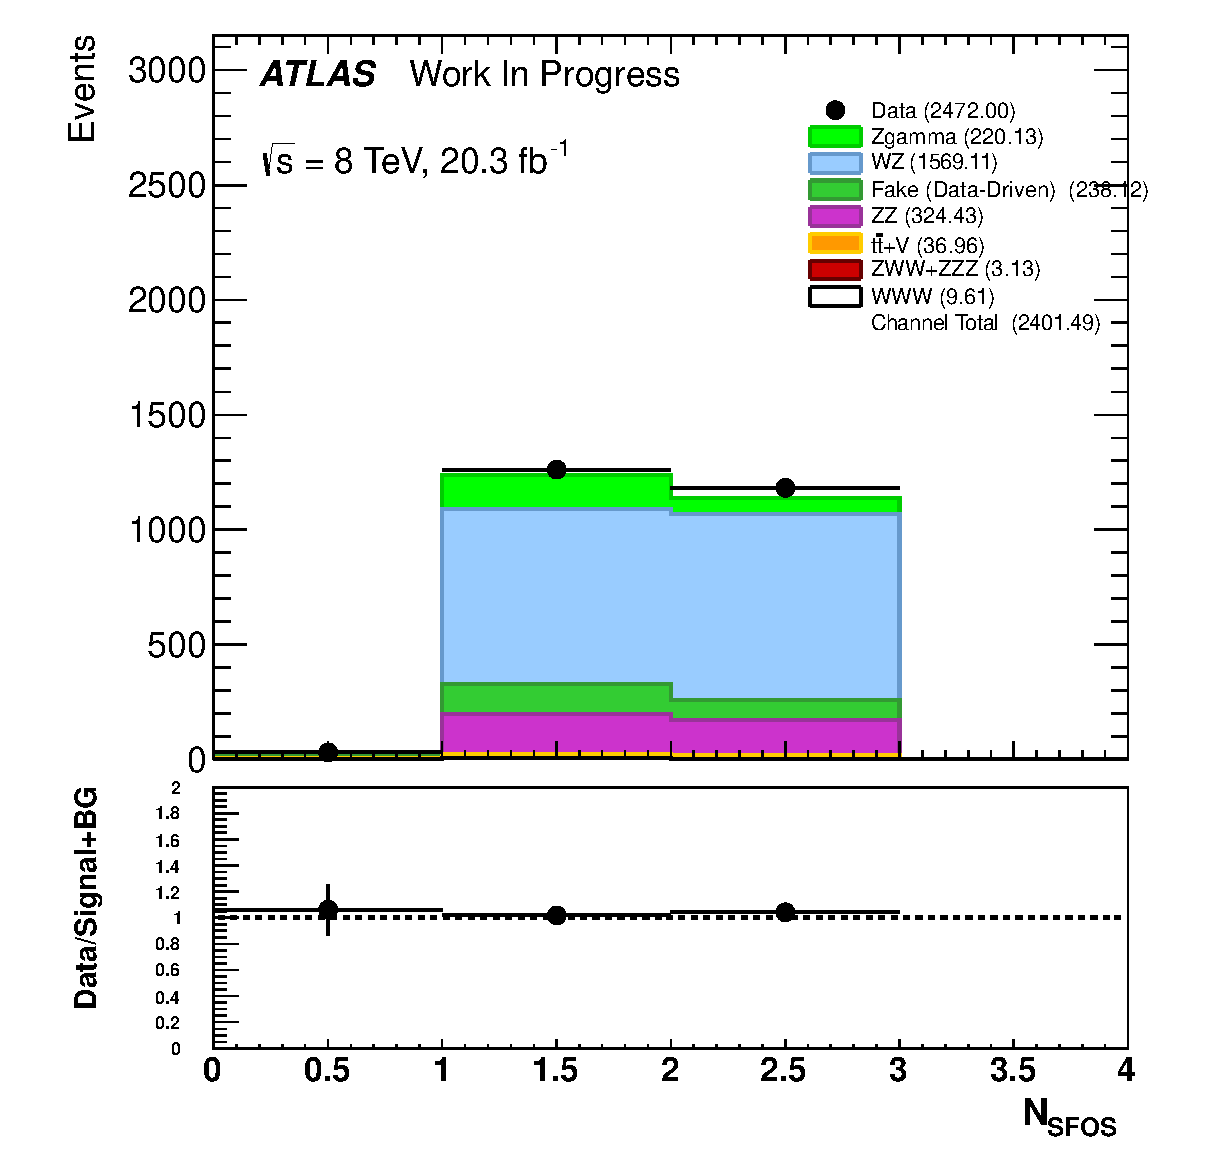
\includegraphics[width=0.3\columnwidth]{figures/preselection/NSFOS_histratio.eps}
%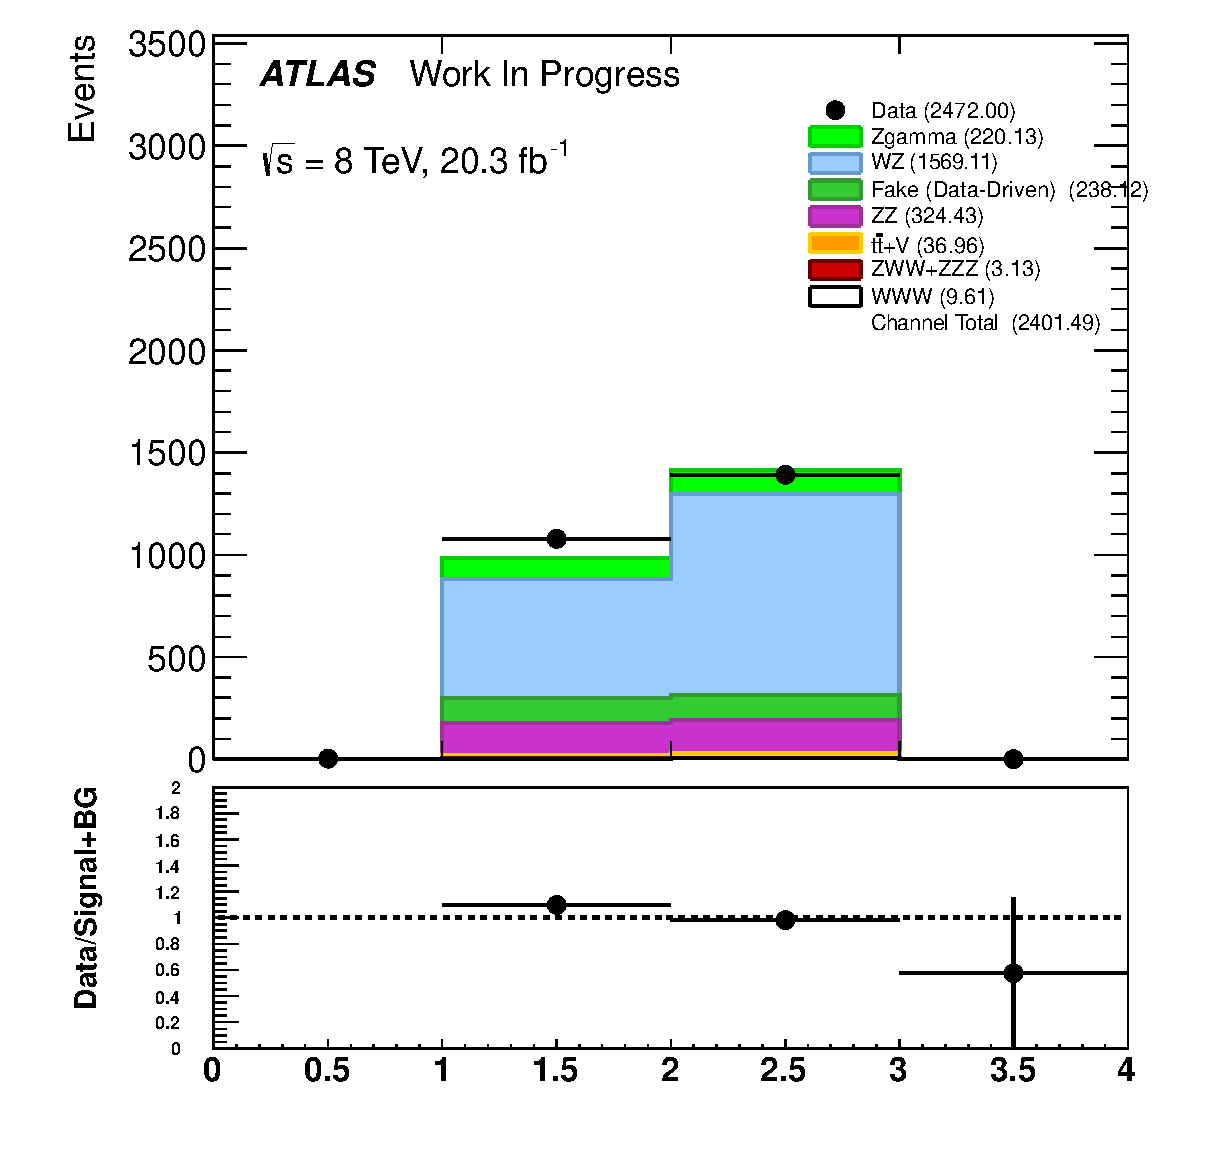
\includegraphics[width=0.3\columnwidth]{figures/preselection/TotalCharge_histratio.eps}
\caption{Distributions showing the observed data compared to the background estimate at event pre-selection.}
\label{fig:preselection}
\end{figure}

\begin{table}[ht!]
\centering
\begin{tabular}{|c||c|c|c|c|}
\hline
 & $eee$ & $ee\mu$ & $e\mu\mu$ & $\mu\mu\mu$\\ 
\hline\hline
$WZ$ &  $240.85 \pm 0.67$ &  $339.17 \pm 0.82$ &  $422.07 \pm 0.87$ &  $567.0 \pm 1$\\ 
$ZZ$ &  $60.21 \pm 0.13$ &  $54.1 \pm 0.2$ &  $118.60 \pm 0.31$ &  $91.48 \pm 0.17$\\ 
$Z\gamma$ &  $70.1 \pm 2.7$ &  $0.47 \pm 0.22$ &  $149.4 \pm 3.9$ &  $0.17 \pm 0.12$\\ 
$ZWW+ZZZ$ &  $0.436 \pm 0.019$ &  $0.834 \pm 0.027$ &  $1.00 \pm 0.03$ &  $0.864 \pm 0.028$\\ 
$t\bar{t}+V$ &  $4.854 \pm 0.044$ &  $9.549 \pm 0.064$ &  $12.047 \pm 0.072$ &  $10.510 \pm 0.066$\\ 
Fake (data-driven) &  $45.1 \pm 2.2$ &  $37.8 \pm 1.6$ &  $112.7 \pm 2.8$ &  $42.5 \pm 1.2$\\ 
$WWW$ &  $0.770 \pm 0.011$ &  $3.023 \pm 0.023$ &  $3.970 \pm 0.026$ &  $1.843 \pm 0.018$\\ 
\hline
Expected Background &  $421.6 \pm 3.5$ &  $441.9 \pm 1.8$ &  $815.8 \pm 4.9$ &  $712.5 \pm 1.6$\\ 
Expected Signal + Background &  $422.4 \pm 3.5$ &  $444.9 \pm 1.8$ &  $819.8 \pm 4.9$ &  $714.4 \pm 1.6$\\ 
\hline
Observed Data &  $426 \pm 21$ &  $468 \pm 22$ &  $821 \pm 29$ &  $757 \pm 28$\\ 
\hline
\end{tabular}

\caption{Expected and observed event yields binned by lepton flavor combination at event pre-selection.
Only statistical uncertainties are shown.
}
\label{tab:preselection}
\end{table}

\begin{figure}[ht!]
\centering
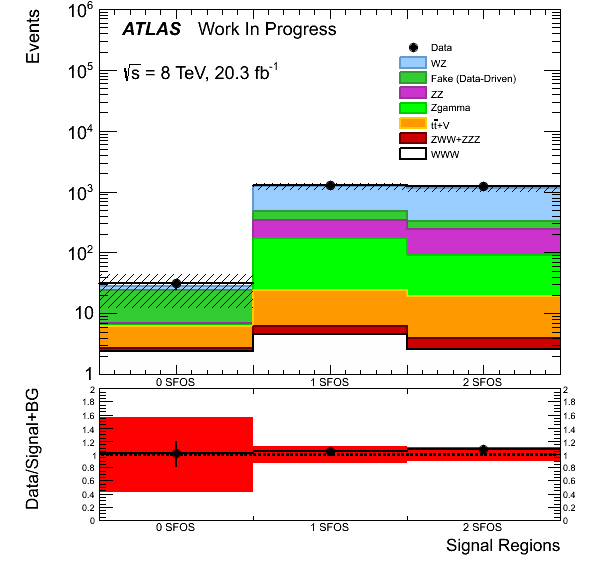
\includegraphics[width=0.5\columnwidth]{figures/preselection/NSFOS_Logy_histratio.png}
%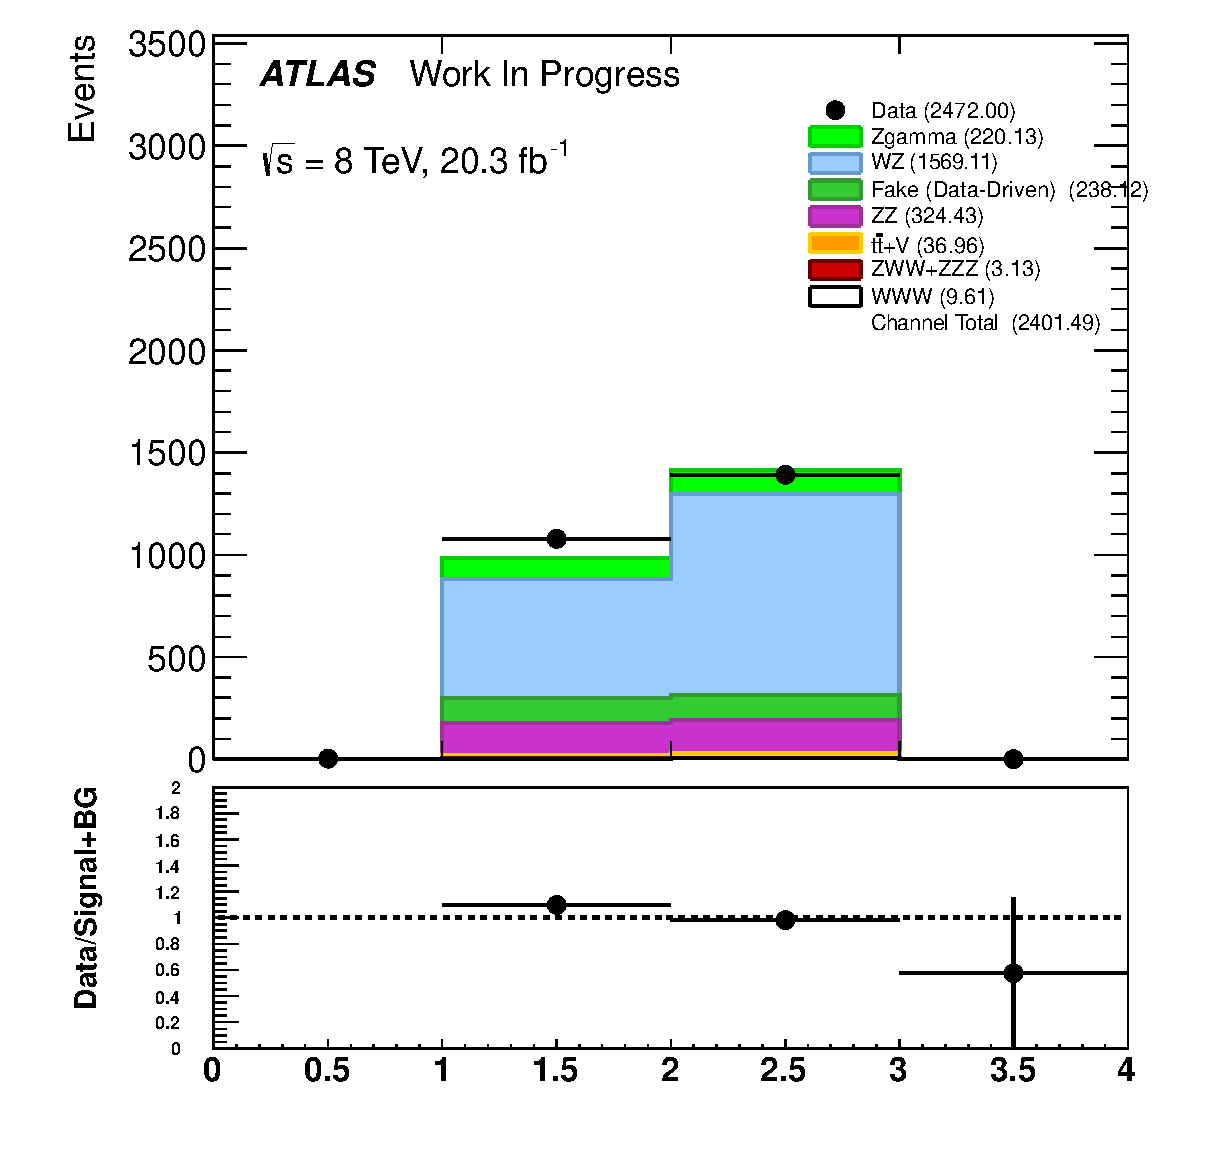
\includegraphics[width=0.3\columnwidth]{figures/preselection/TotalCharge_histratio.eps}
\caption{Yields at event pre-selection in the 0, 1 and 2 SFOS regions.  The most important systematic uncertainties 
(discussed in section~\ref{sec:systematics}) are shown, namely from the fake estimates and the uncertainties on the WZ and ZZ k-factors.}
\label{fig:preselection_nsfos}
\end{figure}

\begin{table}[ht!]
\centering
\begin{tabular}{|c||c|c|c|c|}
\hline
 & $eee$ & $ee\mu$ & $e\mu\mu$ & $\mu\mu\mu$\\ 
\hline\hline
$WZ$ &  $240.85 \pm 0.67$ &  $339.17 \pm 0.82$ &  $422.07 \pm 0.87$ &  $567.0 \pm 1$\\ 
$ZZ$ &  $60.21 \pm 0.13$ &  $54.1 \pm 0.2$ &  $118.60 \pm 0.31$ &  $91.48 \pm 0.17$\\ 
$Z\gamma$ &  $70.1 \pm 2.7$ &  $0.47 \pm 0.22$ &  $149.4 \pm 3.9$ &  $0.17 \pm 0.12$\\ 
$ZWW+ZZZ$ &  $0.436 \pm 0.019$ &  $0.834 \pm 0.027$ &  $1.00 \pm 0.03$ &  $0.864 \pm 0.028$\\ 
$t\bar{t}+V$ &  $4.854 \pm 0.044$ &  $9.549 \pm 0.064$ &  $12.047 \pm 0.072$ &  $10.510 \pm 0.066$\\ 
Fake (data-driven) &  $45.1 \pm 2.2$ &  $37.8 \pm 1.6$ &  $112.7 \pm 2.8$ &  $42.5 \pm 1.2$\\ 
$WWW$ &  $0.770 \pm 0.011$ &  $3.023 \pm 0.023$ &  $3.970 \pm 0.026$ &  $1.843 \pm 0.018$\\ 
\hline
Expected Background &  $421.6 \pm 3.5$ &  $441.9 \pm 1.8$ &  $815.8 \pm 4.9$ &  $712.5 \pm 1.6$\\ 
Expected Signal + Background &  $422.4 \pm 3.5$ &  $444.9 \pm 1.8$ &  $819.8 \pm 4.9$ &  $714.4 \pm 1.6$\\ 
\hline
Observed Data &  $426 \pm 21$ &  $468 \pm 22$ &  $821 \pm 29$ &  $757 \pm 28$\\ 
\hline
\end{tabular}

\caption{Expected and observed event yields binned by lepton flavor combination at event pre-selection.
Only statistical uncertainties are shown.
}
\label{tab:preselection}
\end{table}


\clearpage
\subsection{Signal Regions}
\label{sec:signal_region_yields}
The selection used in the final signal regions is determined as described in Section~\ref{sec:signal_regions} and is summarized in Table~\ref{tab:signal_selection}. Kinematic distributions are shown for the distribution
that is cut on just before the cut is applied
for each stage of the selection in Figures~\ref{fig:0sfos}, \ref{fig:1sfos}, and \ref{fig:2sfos} for
the 0, 1, and 2 SFOS regions, respectively.
A more detailed set of kinematic distributions at each stage of the selection is 
shown in appendix~\ref{sec:app_signal_selection}. 
Cutflows showing the weighted cutflows at each stage of the signal selection are shown for the 0, 1, and 2 SFOS regions
in Tables ~\ref{tab:cutflow_weighted_0sfos}, ~\ref{tab:cutflow_weighted_1sfos}, ~\ref{tab:cutflow_weighted_2sfos}.
Unweighted cutflows are shown in appendix~\ref{sec:app_signal_selection}.

%Tables summarizing the event yields after the final
%selection and binned by the lepton flavor combinations are shown in Tables \ref{tab:0sfos}, \ref{tab:1sfos}, and \ref{tab:2sfos}.




\subsubsection{0 SFOS Signal Region}

The cutflows for the selection in the 0 SFOS region are shown in Table~\ref{tab:cutflow_weighted_0sfos}
while the distributions at each stage of the selection are shown in Figure~\ref{fig:0sfos}.
This is the most sensitive channel with an expected signal to background ratio of 56\%.
The data is observed to agree with the expectation within statstical uncertainties. The background
is ultimately dominated by fake background contributions, which themselves have a large systematic uncertainty
that is similar in size to the statistical uncertainty. This is described in more detail in section~\ref{sec:systematics}.
The poisson probability of observing 5 events with 3.67 events expected from the signal plus background prediction is 14.1\%.


\begin{table}[ht!]
\centering
\scriptsize
\begin{tabular}{l||c|c||c|c||c|c||c|c||c|c||c|c||c|c||c|c}
\hline
 &                 \multicolumn{2}{c||}{Signal}            &  \multicolumn{12}{c||}{Background} &  \multicolumn{2}{c}{Data} \\
 & &  & \multicolumn{2}{c||}{$WZ$} & \multicolumn{2}{c||}{$ZZ$} & \multicolumn{2}{c||}{$t\bar{t}+V$} & \multicolumn{2}{c||}{$ZZZ+ZWW$} & \multicolumn{2}{c||}{$Z\gamma$} & \multicolumn{2}{c||}{Fake} &  & \\ 
 & Yield & Eff. & Yield & Eff. & Yield & Eff. & Yield & Eff. & Yield & Eff. & Yield & Eff. & Yield & Eff. & Yield & Eff.\\
\hline\hline
%1. Pre-selection &  $9.78$ & --- &  $1566.91$ & --- &  $323.60$ &  --- &  $36.93$ &  --- &  $3.12$ & --- &  $219.80$ &  --- &  $238.12$ &  --- & $2472$ &  --- \\ 
%\hline
1. 0 SFOS &  $2.31$ &  --- &  $2.84$ &  --- &  $0.50$ &  --- &  $0.26$ &  --- &  $0.25$ &  --- &  $0.20$ &  --- &  $17.31$ &  --- & $30$ &  ---\\ 
\hline
2. Charge Sum $= \pm 1$ &  $2.30$ &  $1.00$ &  $1.92$ &  $0.68$ &  $0.33$ &  $0.65$ &  $0.26$ &  $0.99$ &  $0.25$ &  $1.00$ &  $0.00$ &  $0.00$ &  $16.79$ &  $0.97$ & $27$ &  $0.90$\\ 
\hline
3. $N_{\mathrm{b-jet}} = 0$ &  $2.29$ &  $0.99$ &  $1.91$ &  $0.99$ &  $0.33$ &  $0.99$ &  $0.25$ &  $0.98$ &  $0.25$ &  $0.99$ &  $0.00$ &  $0.00$ &  $5.85$ &  $0.35$ & $10$ &  $0.37$\\ 
\hline
4. $m_{SF} > 20$ GeV &  $2.25$ &  $0.98$ &  $1.88$ &  $0.98$ &  $0.32$ &  $0.98$ &  $0.25$ &  $0.98$ &  $0.24$ &  $0.98$ &  $0.00$ &  $0.00$ &  $5.63$ &  $0.96$ & $10$ &  $1.00$\\ 
\hline
5. $|m_{ee} - m_{Z}| > 15$ GeV &  $2.06$ &  $0.91$ &  $1.27$ &  $0.68$ &  $0.21$ &  $0.66$ &  $0.22$ &  $0.90$ &  $0.22$ &  $0.90$ &  $0.00$ &  $0.00$ &  $5.17$ &  $0.92$ & $9$ &  $0.90$\\ 
\hline
6. $|\Delta\phi(3l,E_{T}^{Miss})| > 2.5$ &  $1.41$ &  $0.69$ &  $0.65$ &  $0.51$ &  $0.07$ &  $0.34$ &  $0.09$ &  $0.38$ &  $0.13$ &  $0.59$ &  $0.00$ &  $0.00$ &  $2.17$ &  $0.42$ & $6$ &  $0.67$\\ 
\hline
7. $N_{\mathrm{Jet}} \leq 1$ &  $1.34$ &  $0.95$ &  $0.62$ &  $0.95$ &  $0.07$ &  $0.91$ &  $0.04$ &  $0.45$ &  $0.11$ &  $0.86$ &  $0.00$ &  $0.00$ &  $1.51$ &  $0.70$ & $5$ &  $0.83$\\ 
\hline
\end{tabular}




\caption{Cutflows showing the event yields and efficiencies for each cut in the 0 SFOS signal region
starting from event pre-selection and binned by category. 
Event yields for MC backgrounds and signal include all weights and are normalized to an integrated luminosity of $20.3~\mathrm{fb}^{-1}$.  
The fake lepton background only includes the matrix method weights.  The data is unweighted.
Efficiencies show the ratio of the yield with respect
to the previous cut.  The efficiency is first calculated at the first cut after event pre-selection.  }
\label{tab:cutflow_weighted_0sfos}
\end{table}



%0 SFOS, consolidated
\begin{figure}[ht!]
\centering
%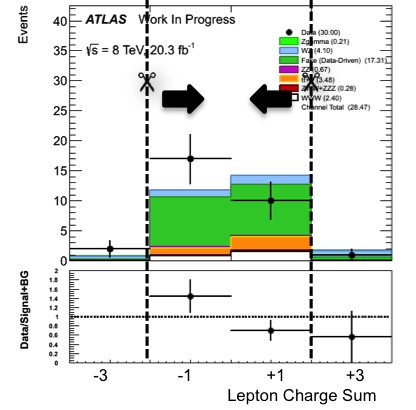
\includegraphics[width=0.3\columnwidth]{figures/cuts/0sfos_charge_sum.png}
%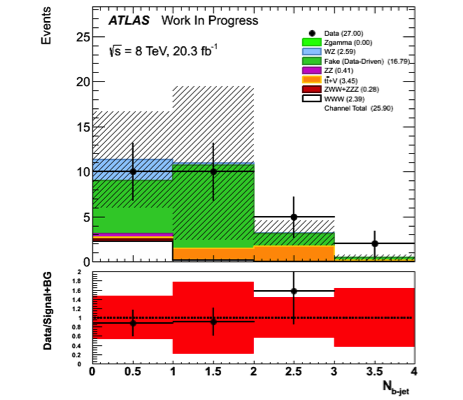
\includegraphics[width=0.3\columnwidth]{figures/cuts/0sfos_chargesum_bjet.png}
%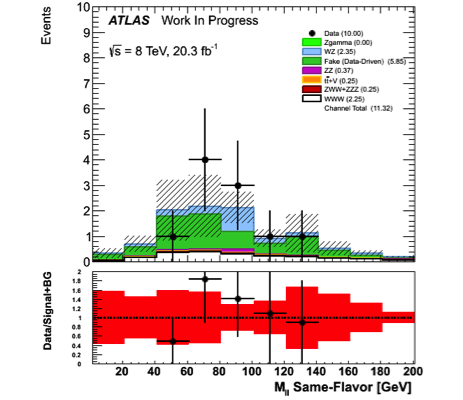
\includegraphics[width=0.3\columnwidth]{figures/cuts/0sfos_chargesum_bjet_msf.png}
%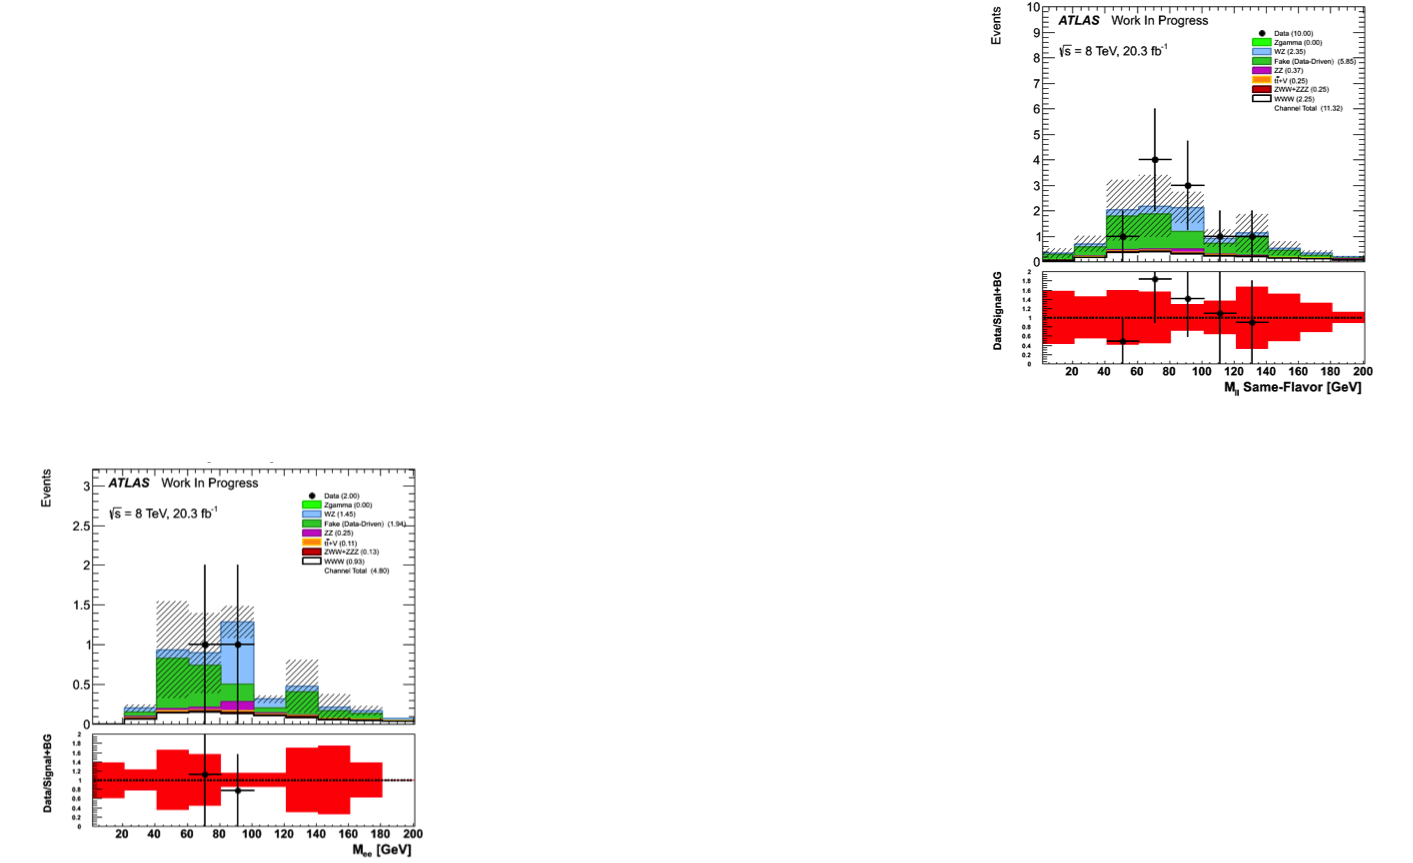
\includegraphics[width=0.3\columnwidth]{figures/cuts/0sfos_chargesum_bjet_msf_mee.png}
%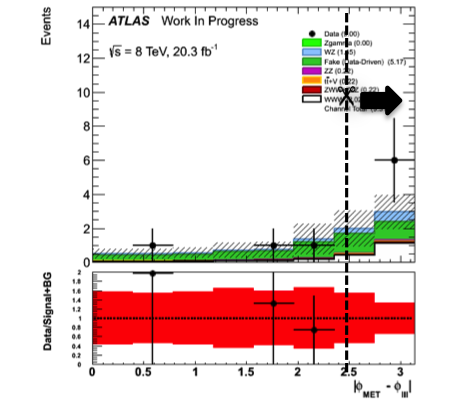
\includegraphics[width=0.3\columnwidth]{figures/cuts/0sfos_chargesum_bjet_msf_mee_deltaphi.png}
%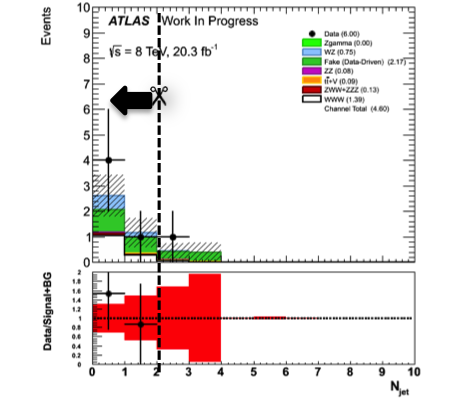
\includegraphics[width=0.3\columnwidth]{figures/cuts/0sfos_chargesum_bjet_msf_mee_deltaphi_njet.png}
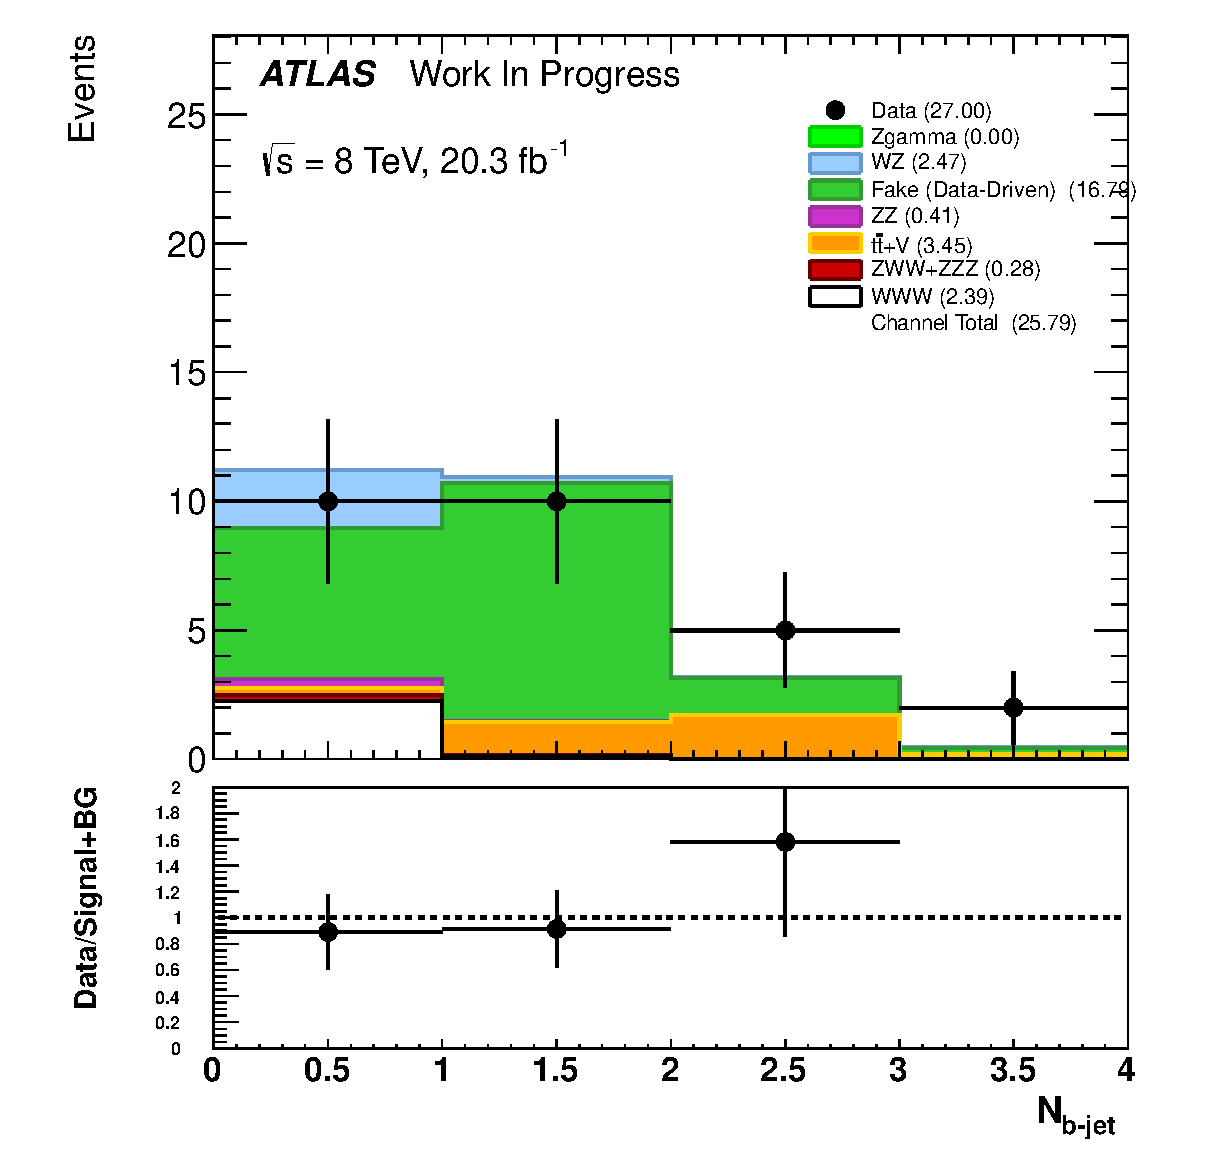
\includegraphics[width=0.3\columnwidth]{figures/appendix_signal_selection/PreselectionJune2_NoSTVF_0SFOS_ChargeAbs1_physics/weight_all/eps/NBTaggedJets_histratio.eps}
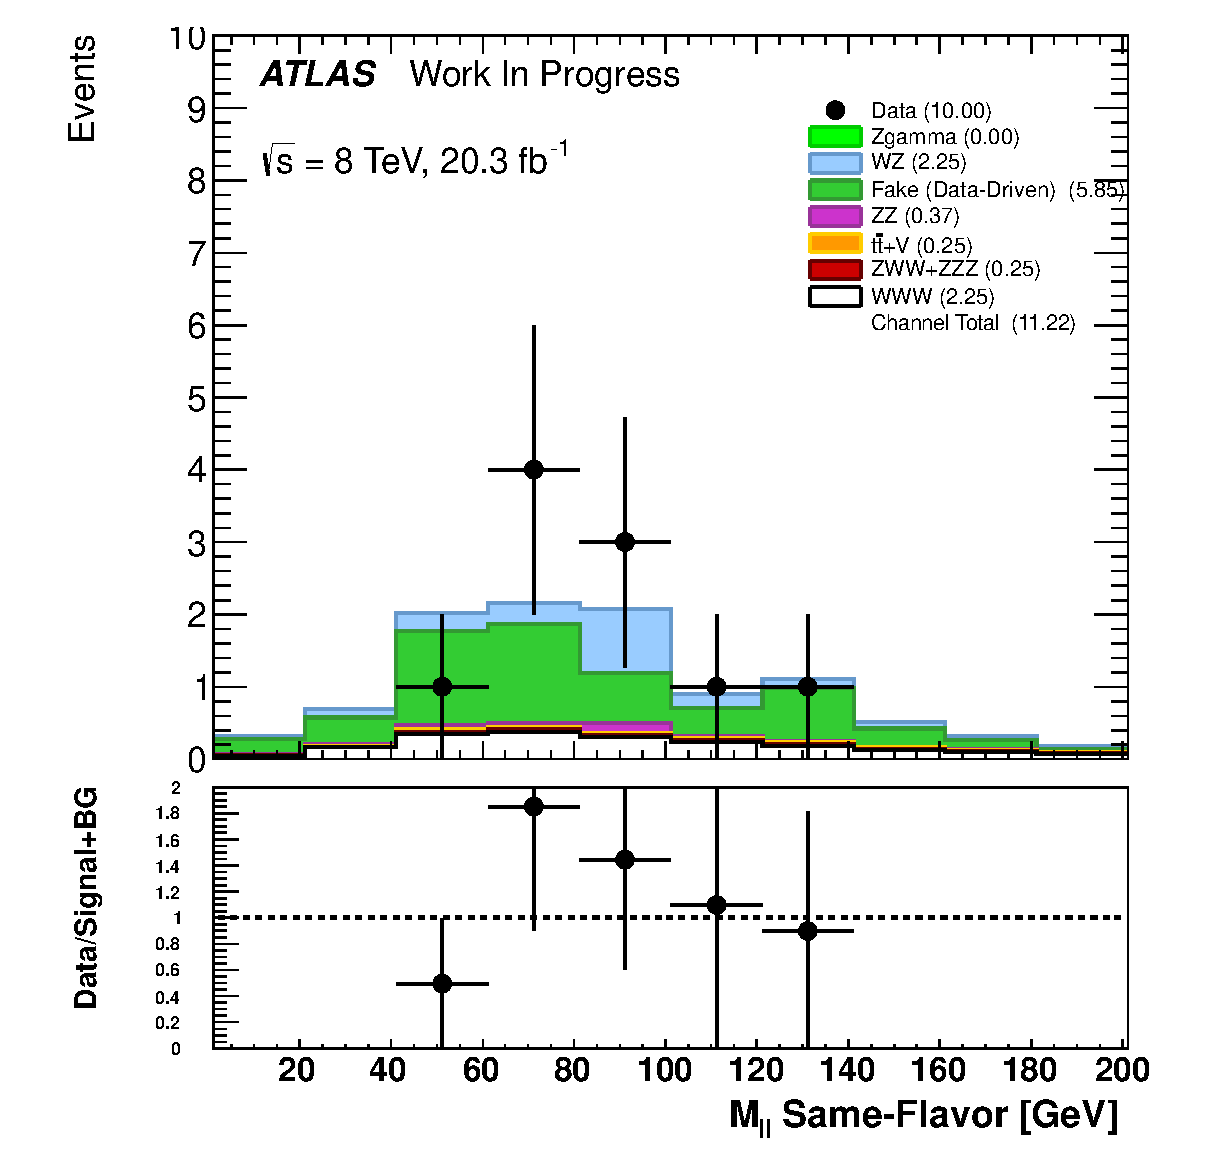
\includegraphics[width=0.3\columnwidth]{figures/appendix_signal_selection/PreselectionJune2_NoSTVF_0SFOS_ChargeAbs1_BVeto85_physics/weight_all/eps/InvariantMassSF_histratio.eps}
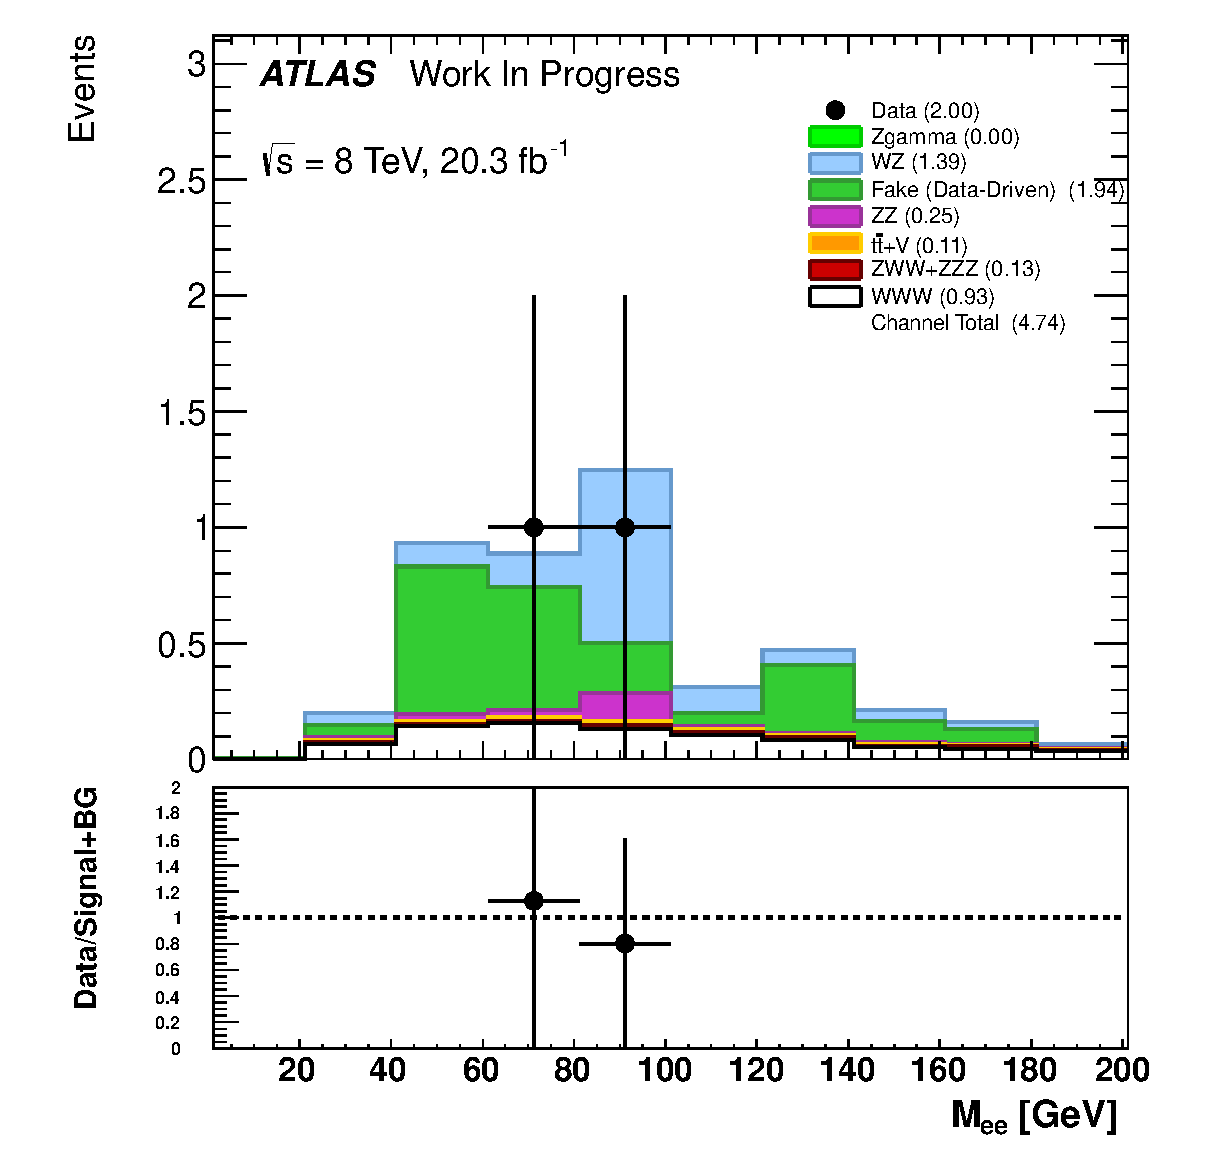
\includegraphics[width=0.3\columnwidth]{figures/appendix_signal_selection/PreselectionJune2_NoSTVF_0SFOS_ChargeAbs1_BVeto85_SFMllGt20_physics/weight_all/eps/InvariantMassElEl_histratio.eps}
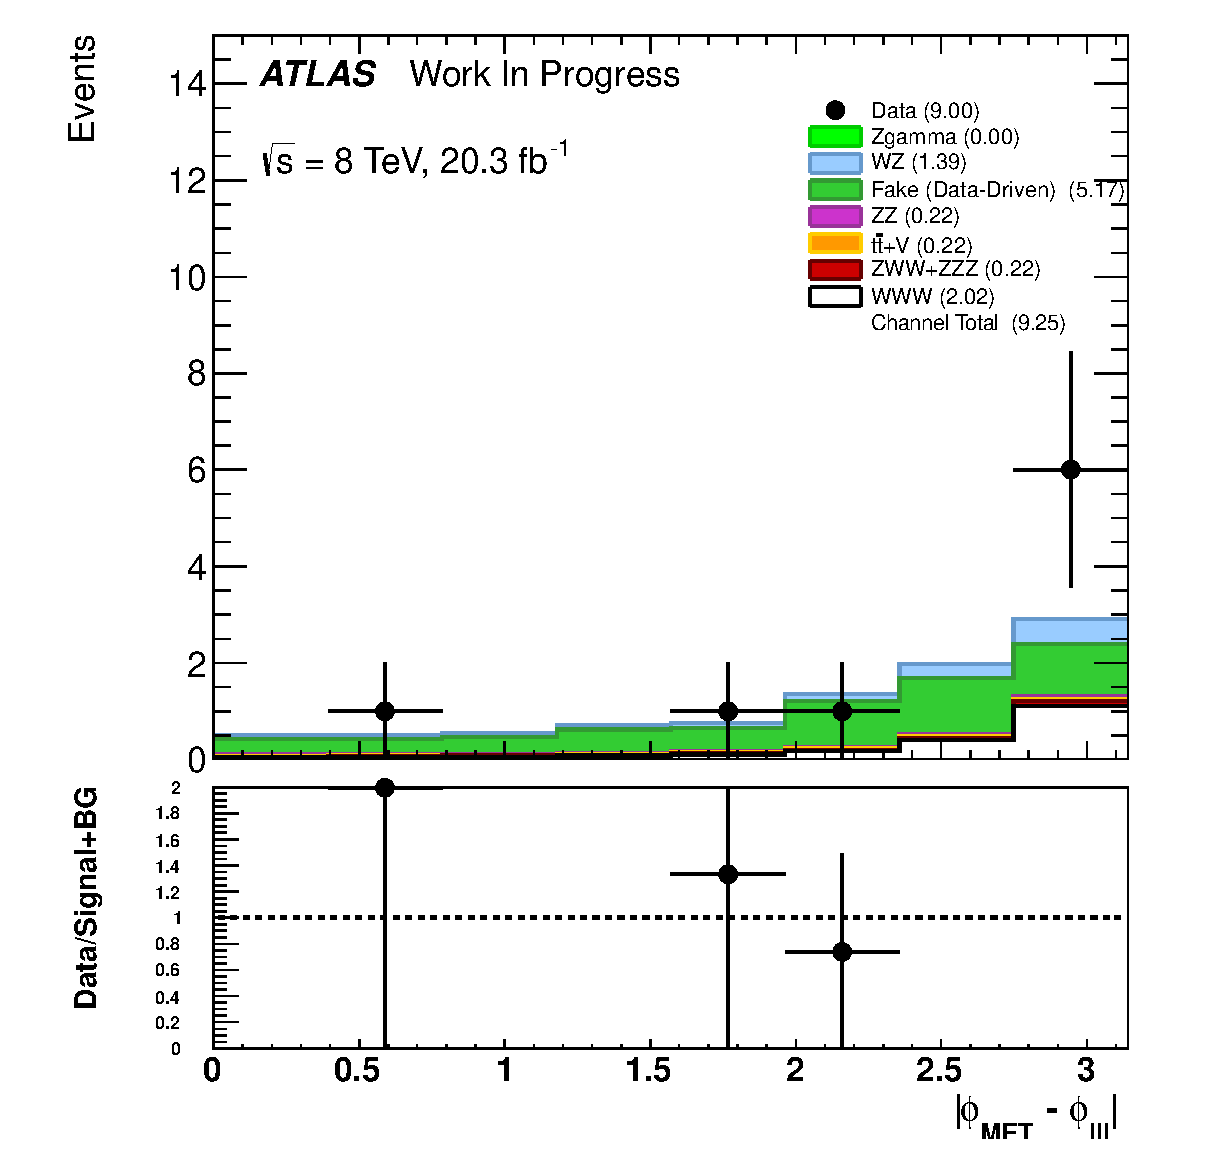
\includegraphics[width=0.3\columnwidth]{figures/appendix_signal_selection/PreselectionJune2_NoSTVF_0SFOS_ChargeAbs1_BVeto85_SFMllGt20_SSMeeZVeto15_physics/weight_all/eps/DeltaPhiMET123_Abs_histratio.eps}
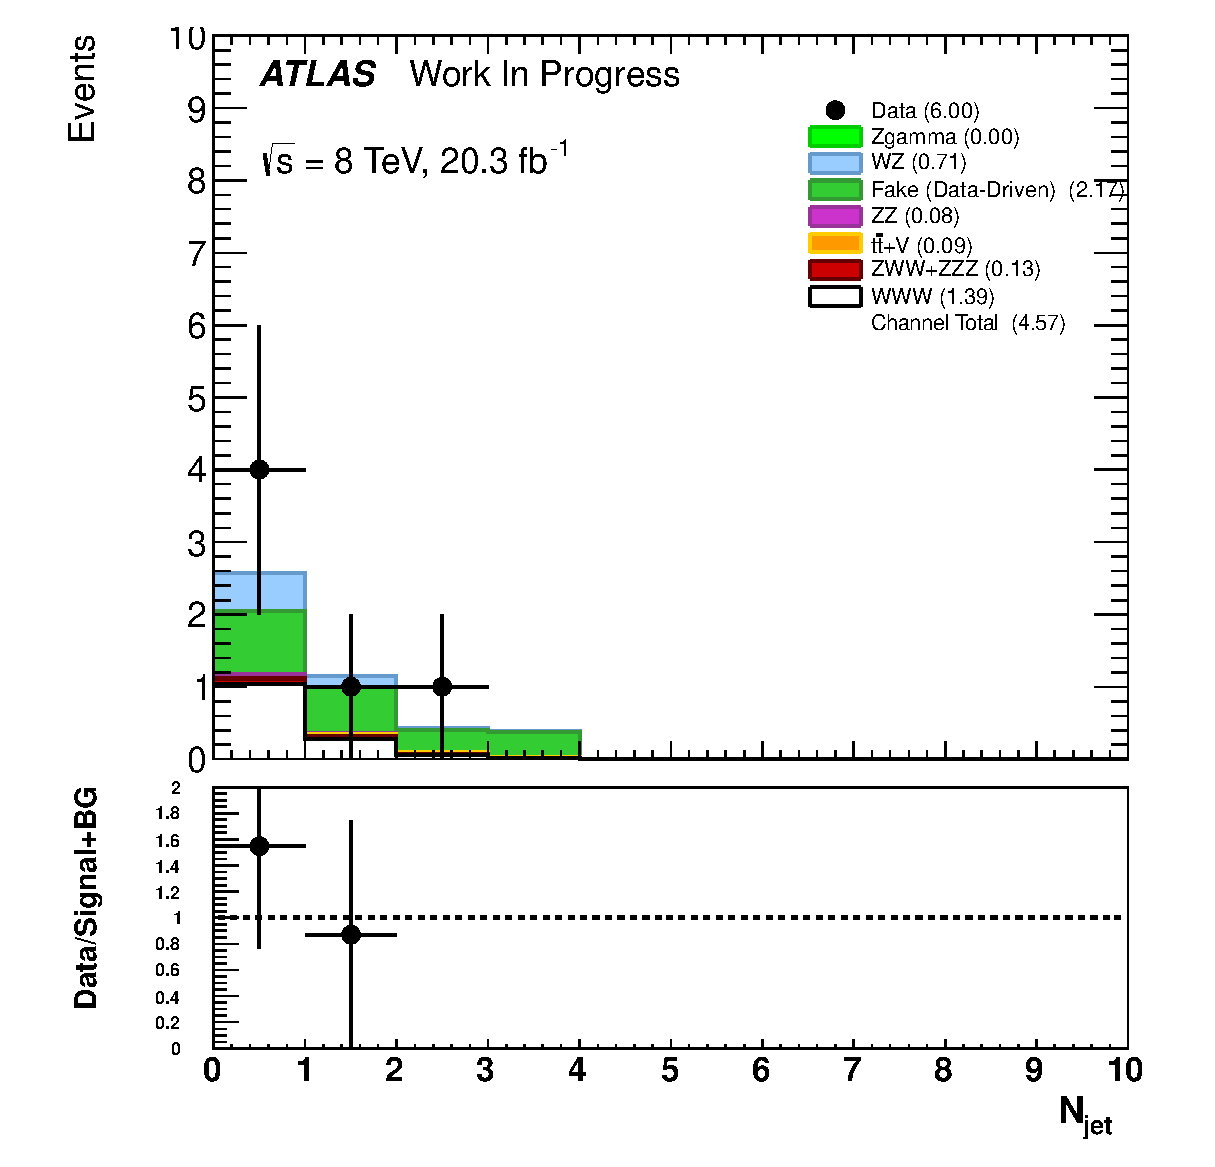
\includegraphics[width=0.3\columnwidth]{figures/appendix_signal_selection/PreselectionJune2_NoSTVF_0SFOS_ChargeAbs1_BVeto85_SFMllGt20_SSMeeZVeto15_DeltaPhi2p5_physics/weight_all/eps/NJets_histratio.eps}
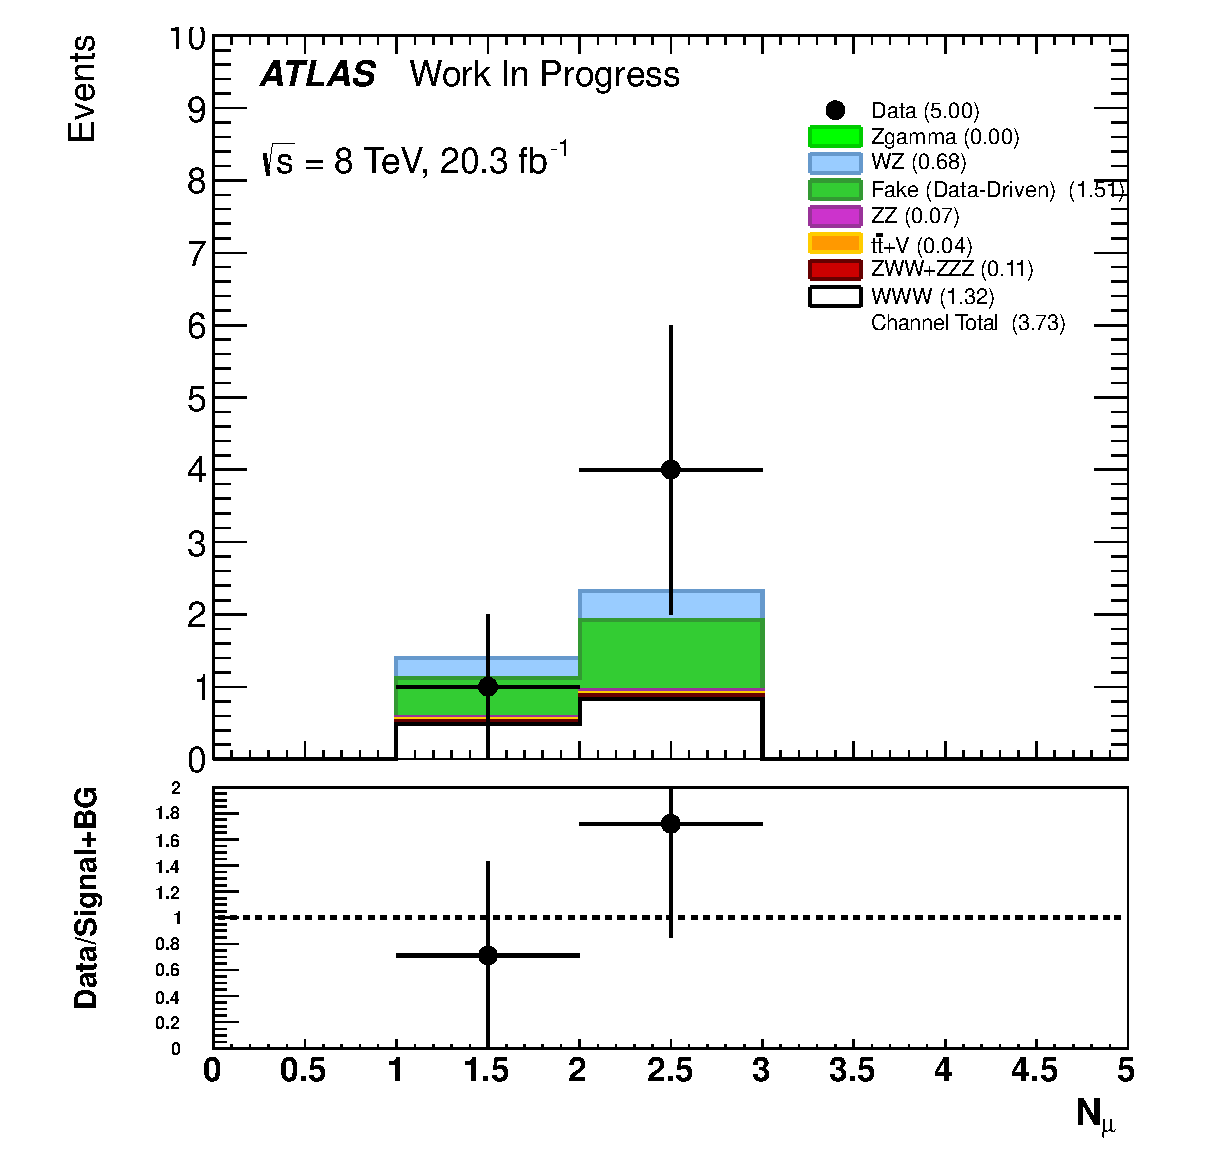
\includegraphics[width=0.3\columnwidth]{figures/appendix_signal_selection/PreselectionJune2_NoSTVF_0SFOS_ChargeAbs1_BVeto85_SFMllGt20_SSMeeZVeto15_DeltaPhi2p5_NJetLt2_physics/weight_all/eps/NMuons_histratio.eps}
\caption{Distributions showing data compared to the signal plus background estimate in the 0 SFOS region at each stage 
of the selection before the cuts are applied to the given distribution. 
Plots should be read sequentially from left to right
and from top to bottom. 
Referring to Table~\ref{tab:cutflow_weighted_0sfos}, the top left
plot is shown before cut \#4 is applied, top middle is before cut \#5, and
so on until the bottom right which is after all cuts are applied.
}
\label{fig:0sfos}
\end{figure}

%\begin{table}[ht!]
%\centering
%\begin{tabular}{|c||c|c|c|c|}
\hline
 & $eee$ & $ee\mu$ & $e\mu\mu$ & $\mu\mu\mu$\\ 
\hline\hline
$WZ$ &  $0.0 \pm 0$ &  $0.279 \pm 0.011$ &  $0.3976 \pm 0.0071$ &  $0.0 \pm 0$\\ 
$ZZ$ &  $0.0 \pm 0$ &  $0.0283 \pm 0.0022$ &  $0.0410 \pm 0.0037$ &  $0.0 \pm 0$\\ 
$Z\gamma$ &  $0.0 \pm 0$ &  $0.0 \pm 0$ &  $0.0 \pm 0$ &  $0.0 \pm 0$\\ 
$ZWW+ZZZ$ &  $0.0 \pm 0$ &  $0.0496 \pm 0.0067$ &  $0.0630 \pm 0.0074$ &  $0.0 \pm 0$\\ 
$t\bar{t}+V$ &  $0.0 \pm 0$ &  $0.0149 \pm 0.0027$ &  $0.0239 \pm 0.0033$ &  $0.0 \pm 0$\\ 
Fake (data-driven) &  $0.0 \pm 0$ &  $0.55 \pm 0.19$ &  $0.97 \pm 0.17$ &  $0.0 \pm 0$\\ 
$WWW$ &  $0.0 \pm 0$ &  $0.4879 \pm 0.0091$ &  $0.832 \pm 0.012$ &  $0.0 \pm 0$\\ 
\hline
Expected Background &  $0.0 \pm 0$ &  $0.92 \pm 0.19$ &  $1.49 \pm 0.17$ &  $0.0 \pm 0$\\ 
Expected Signal + Background &  $0.0 \pm 0$ &  $1.40 \pm 0.19$ &  $2.33 \pm 0.17$ &  $0.0 \pm 0$\\ 
\hline
Observed Data &  $0.0 \pm 0$ &  $1.0 \pm 1$ &  $4.0 \pm 2$ &  $0.0 \pm 0$\\ 
\hline
\end{tabular}

%\caption{ Expected and observed event yields binned by lepton flavor combination for the optimized 0 SFOS signal region selection defined as follows: event pre-selection + 0 SFOS + charge sum $=\pm1$ + b-veto + $m_{SF}$ + Same-Sign Z-veto + $\Delta\phi$ + $N_{jet}$.
%Only statistical uncertainties are shown.
%}
%\label{tab:0sfos}
%\end{table}


\clearpage
\subsubsection{1 SFOS Signal Region}
The cutflows for the selection in the 1 SFOS region are shown in Table~\ref{tab:cutflow_weighted_1sfos}
while the distributions at each stage of the selection are shown in Figure~\ref{fig:1sfos}.
This region is not as sensitive as the 0 SFOS region with a signal to background ratio of about 9.2\%.
The background is overwhelmingly dominated by $WZ$ contributions. The observed data is slightly discrepant
from the overall prediction, but is about 1 sigma if considering systematics, as demonstrated later in Table~\ref{tab:sys_summary}.
The difference is observed to come almost entirely from the $ee\mu$ region, while the $e\mu\mu$ region shows good agreement, as can
be seen in the bottom right of Figure~\ref{fig:1sfos}. From Figure~\ref{fig:1sfos} we can also see that the agreement
is quite good at each stage of the selection until the cut on the jet multiplicity (bottom middle of Figure~\ref{fig:1sfos}) where the 0 and 1 jet
bins are kept but the 1 jet bin is discrepant.  This suggests that the discrepancy comes from this cut.  This was investigated further
for the different lepton flavor combinations in appendix~\ref{sec:app_signal_selection}.  The efficiencies for the predictions
are very similar for the jet multiplicity cut between the two lepton flavor bins. However, there is a smaller efficiency observed
in the data in the $ee\mu$ bin.  This suggests that the difference is most likely due to a statistical fluctuation.
The poisson probability of observing 13 events with 16.14 events expected from the signal plus background prediction is 7.9\%.

\begin{table}[ht!]
\centering
\scriptsize
\begin{tabular}{l||c|c||c|c||c|c||c|c||c|c||c|c||c|c||c|c}
\hline
 &                 \multicolumn{2}{c||}{Signal}            &  \multicolumn{12}{c||}{Background} &  \multicolumn{2}{c}{Data} \\
 & &  & \multicolumn{2}{c||}{$WZ$} & \multicolumn{2}{c||}{$ZZ$} & \multicolumn{2}{c||}{$t\bar{t}+V$} & \multicolumn{2}{c||}{$ZZZ+ZWW$} & \multicolumn{2}{c||}{$Z\gamma$} & \multicolumn{2}{c||}{Fake} &  & \\ 
 & Yield & Eff. & Yield & Eff. & Yield & Eff. & Yield & Eff. & Yield & Eff. & Yield & Eff. & Yield & Eff. & Yield & Eff.\\
\hline\hline
1. Pre-selection &  $9.78$ & --- &  $1566.91$ & --- &  $323.60$ & --- &  $36.93$ & --- &  $3.12$ & --- &  $219.80$ & --- &  $238.12$ & ---  & $2472$ &  --- \\
\hline
2. 1 SFOS &  $4.67$ &  $0.48$ &  $757.38$ &  $0.48$ &  $171.39$ &  $0.53$ &  $18.10$ &  $0.49$ &  $1.55$ &  $0.50$ &  $149.60$ &  $0.68$ &  $133.47$ &  $0.56$ & $1260$ &  $0.51$\\ 
\hline
3. $N_{\mathrm{b-jet}} = 0$ &  $4.42$ &  $0.94$ &  $696.90$ &  $0.92$ &  $150.14$ &  $0.88$ &  $1.42$ &  $0.08$ &  $1.31$ &  $0.84$ &  $136.96$ &  $0.92$ &  $99.93$ &  $0.75$ & $1095$ &  $0.87$\\ 
\hline
%NOT $m_Z - 35~\mathrm{GeV} < m_{\mathrm{SFOS}} < m_Z + 20~\mathrm{GeV}$ &  $2.71$ &  $0.63$ &  $44.30$ &  $0.06$ &  $13.79$ &  $0.09$ &  $0.37$ &  $0.26$ &  $0.34$ &  $0.26$ &  $22.44$ &  $0.16$ &  $16.72$ &  $0.17$\\ 
4. NOT $m_Z - 35~\mathrm{GeV} <$  &  \multirow{2}{*}{$2.76$} &  \multirow{2}{*}{$0.63$} &  \multirow{2}{*}{$44.30$} &  \multirow{2}{*}{$0.06$} &  \multirow{2}{*}{$13.79$} &  \multirow{2}{*}{$0.09$} &  \multirow{2}{*}{$0.37$} &  \multirow{2}{*}{$0.26$} &  \multirow{2}{*}{$0.34$} &  \multirow{2}{*}{$0.26$} &  \multirow{2}{*}{$22.44$} &  \multirow{2}{*}{$0.16$} &  \multirow{2}{*}{$16.72$} &  \multirow{2}{*}{$0.17$} & \multirow{2}{*}{$93$} &  \multirow{2}{*}{$0.08$}\\ 
$ m_{\mathrm{SFOS}} < m_Z + 20~\mathrm{GeV}$  & & & & & & & & & & & & & &  & \\
\hline
5. $E_{T}^{Miss} > 45$ GeV &  $1.91$ &  $0.69$ &  $21.38$ &  $0.48$ &  $1.46$ &  $0.11$ &  $0.29$ &  $0.78$ &  $0.24$ &  $0.71$ &  $1.36$ &  $0.06$ &  $5.10$ &  $0.31$ & $27$ &  $0.29$\\ 
\hline
6. $|\Delta\phi(3l,E_{T}^{Miss})| > 2.5$ &  $1.48$ &  $0.77$ &  $13.07$ &  $0.61$ &  $0.71$ &  $0.49$ &  $0.11$ &  $0.39$ &  $0.17$ &  $0.69$ &  $0.20$ &  $0.15$ &  $2.47$ &  $0.48$ & $16$ &  $0.59$\\ 
\hline
7. $N_{\mathrm{Jet}} \leq 1$ &  $1.39$ &  $0.94$ &  $11.90$ &  $0.91$ &  $0.58$ &  $0.82$ &  $0.05$ &  $0.45$ &  $0.14$ &  $0.84$ &  $0.20$ &  $1.00$ &  $1.90$ &  $0.77$ & $13$ &  $0.81$\\ 
\hline
\end{tabular}

\caption{Cutflows showing the event yields and efficiencies for each cut in the 1 SFOS signal region
starting from event pre-selection and binned by category. 
Event yields for MC backgrounds and signal include all weights and are normalized to an integrated luminosity of $20.3~\mathrm{fb}^{-1}$.  
The fake lepton background only includes the matrix method weights.  The data is unweighted.
Efficiencies show the ratio of the yield with respect
to the previous cut.  The efficiency is first calculated at the first cut after event pre-selection.  }
\label{tab:cutflow_weighted_1sfos}
\end{table}



%1 SFOS consolidated
\begin{figure}[ht!]
\centering
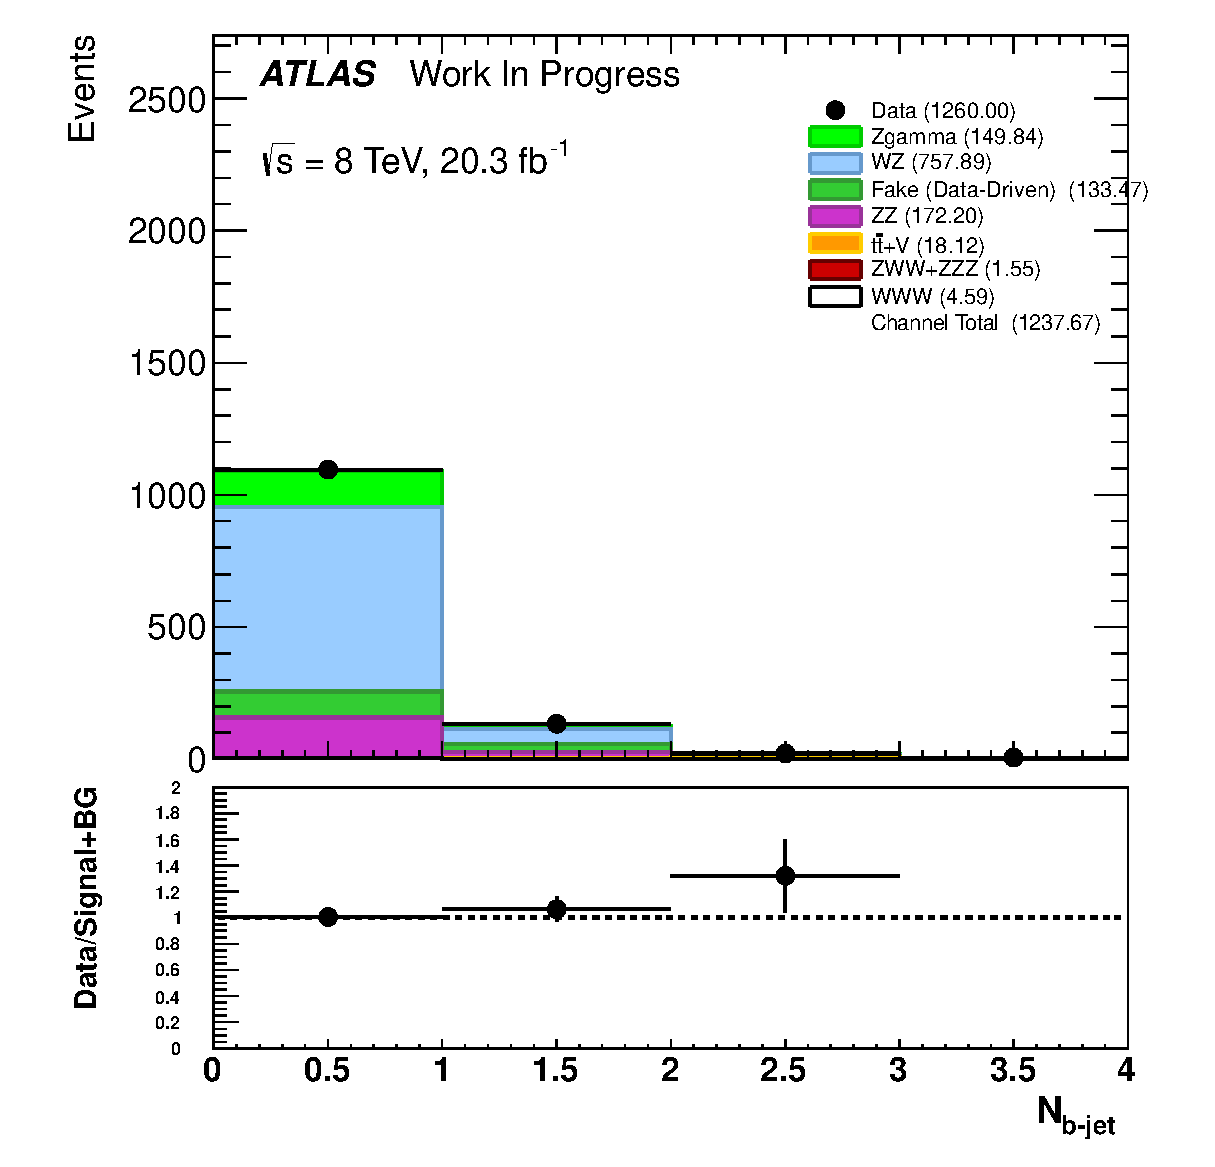
\includegraphics[width=0.3\columnwidth]{figures/appendix_signal_selection/PreselectionMay29_1SFOS_ChargeAbs1_physics/weight_all/eps/NBTaggedJets_histratio.eps}
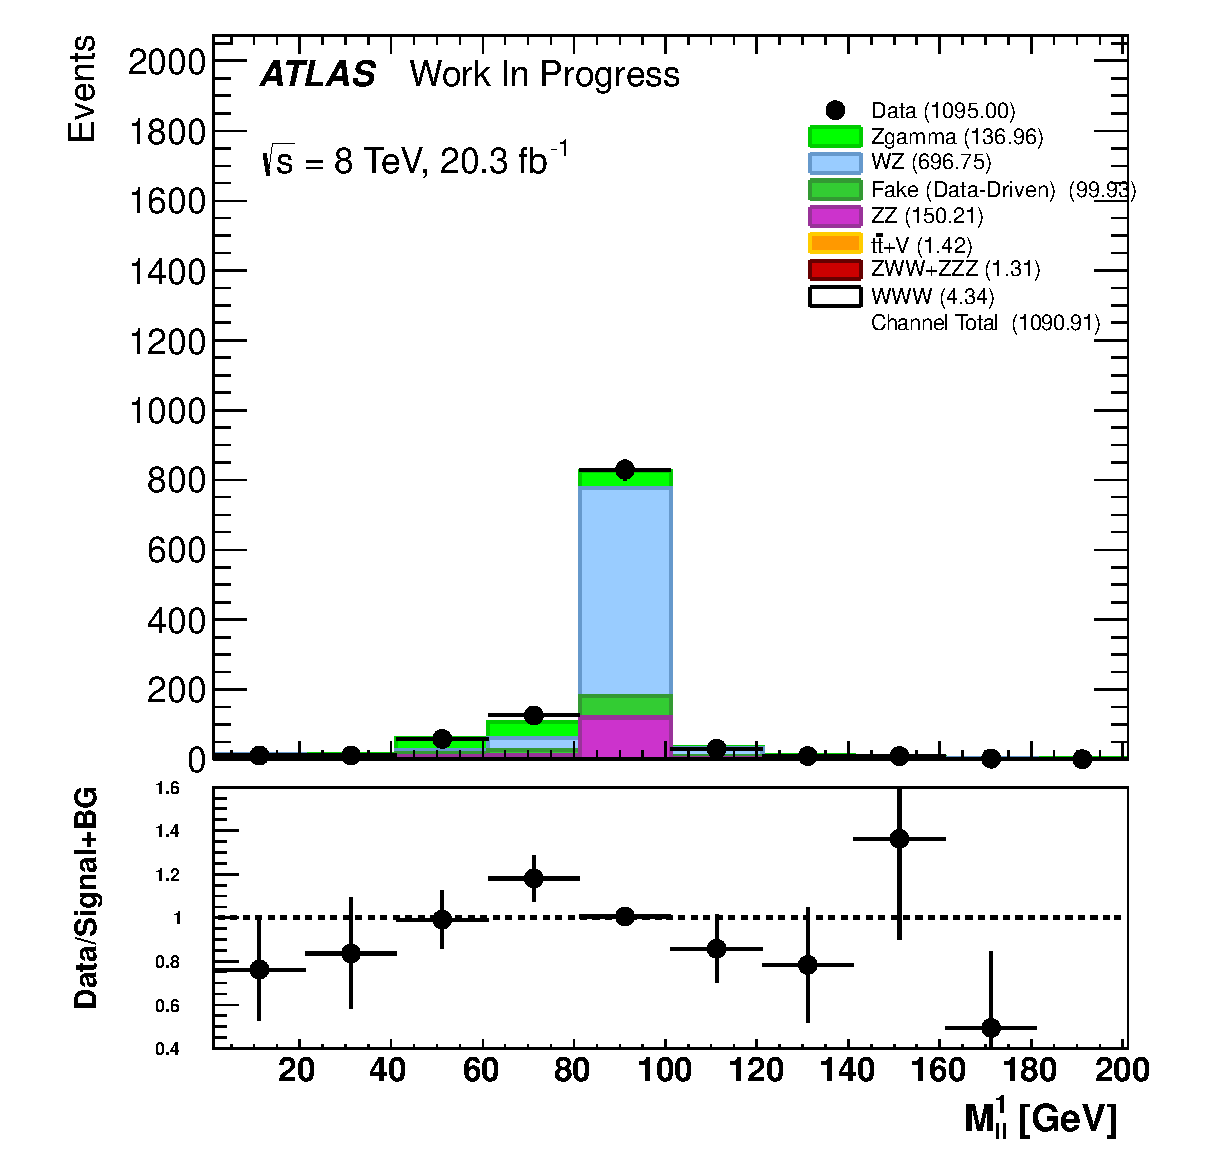
\includegraphics[width=0.3\columnwidth]{figures/appendix_signal_selection/PreselectionMay29_1SFOS_ChargeAbs1_BVeto85_physics/weight_all/eps/InvariantMassSFOS_histratio.eps}
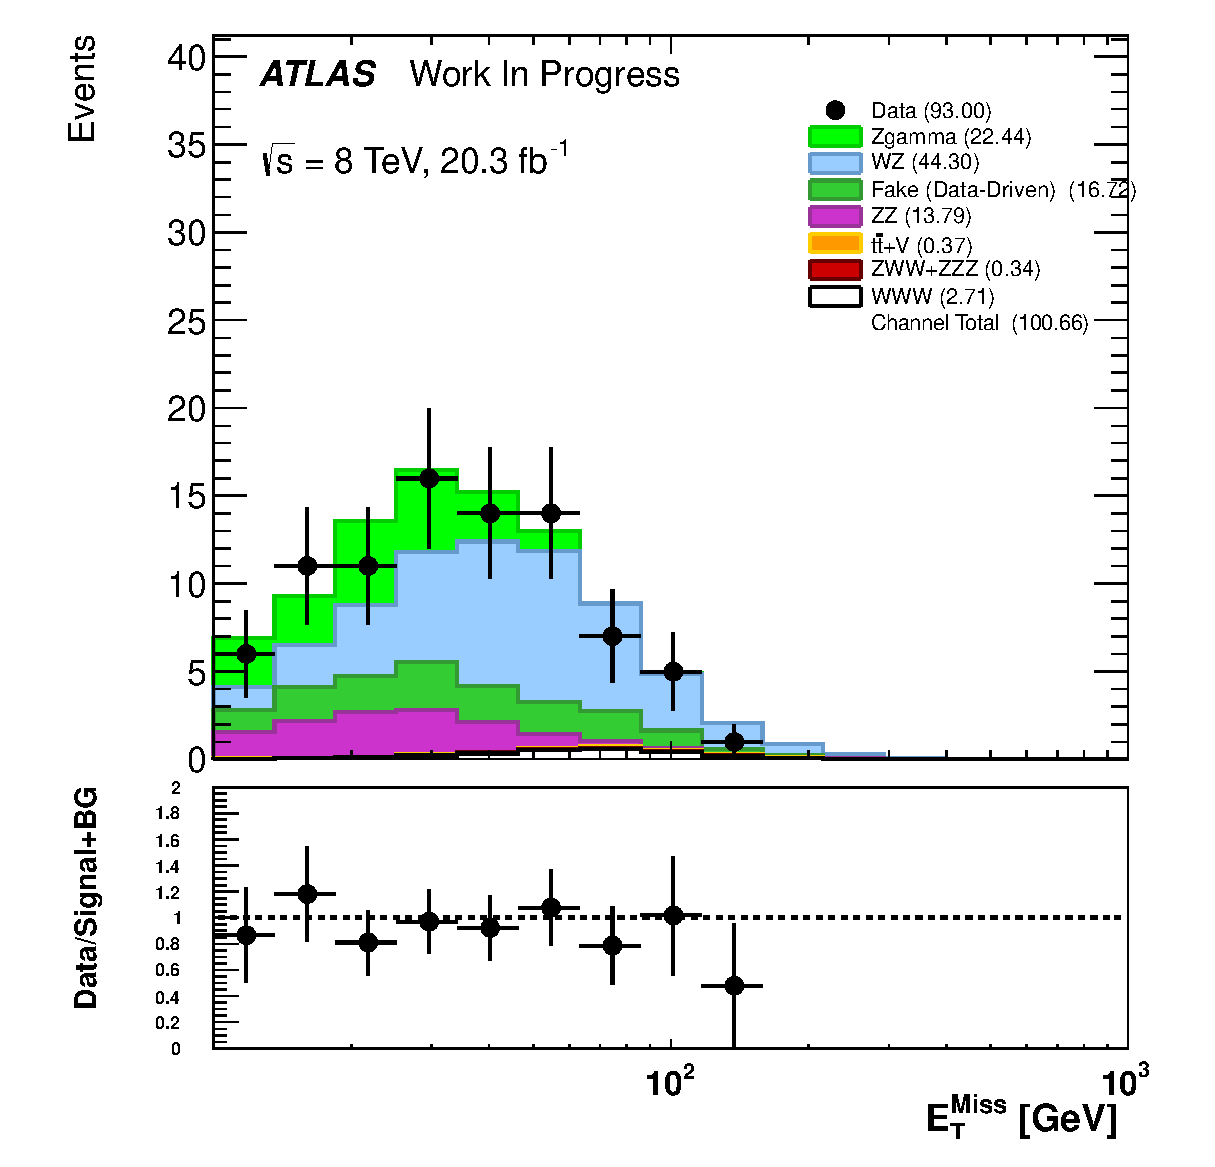
\includegraphics[width=0.3\columnwidth]{figures/appendix_signal_selection/PreselectionMay29_1SFOS_ChargeAbs1_ZVetoLow35High25GeV_physics/weight_all/eps/MET_Et_histratio.eps}
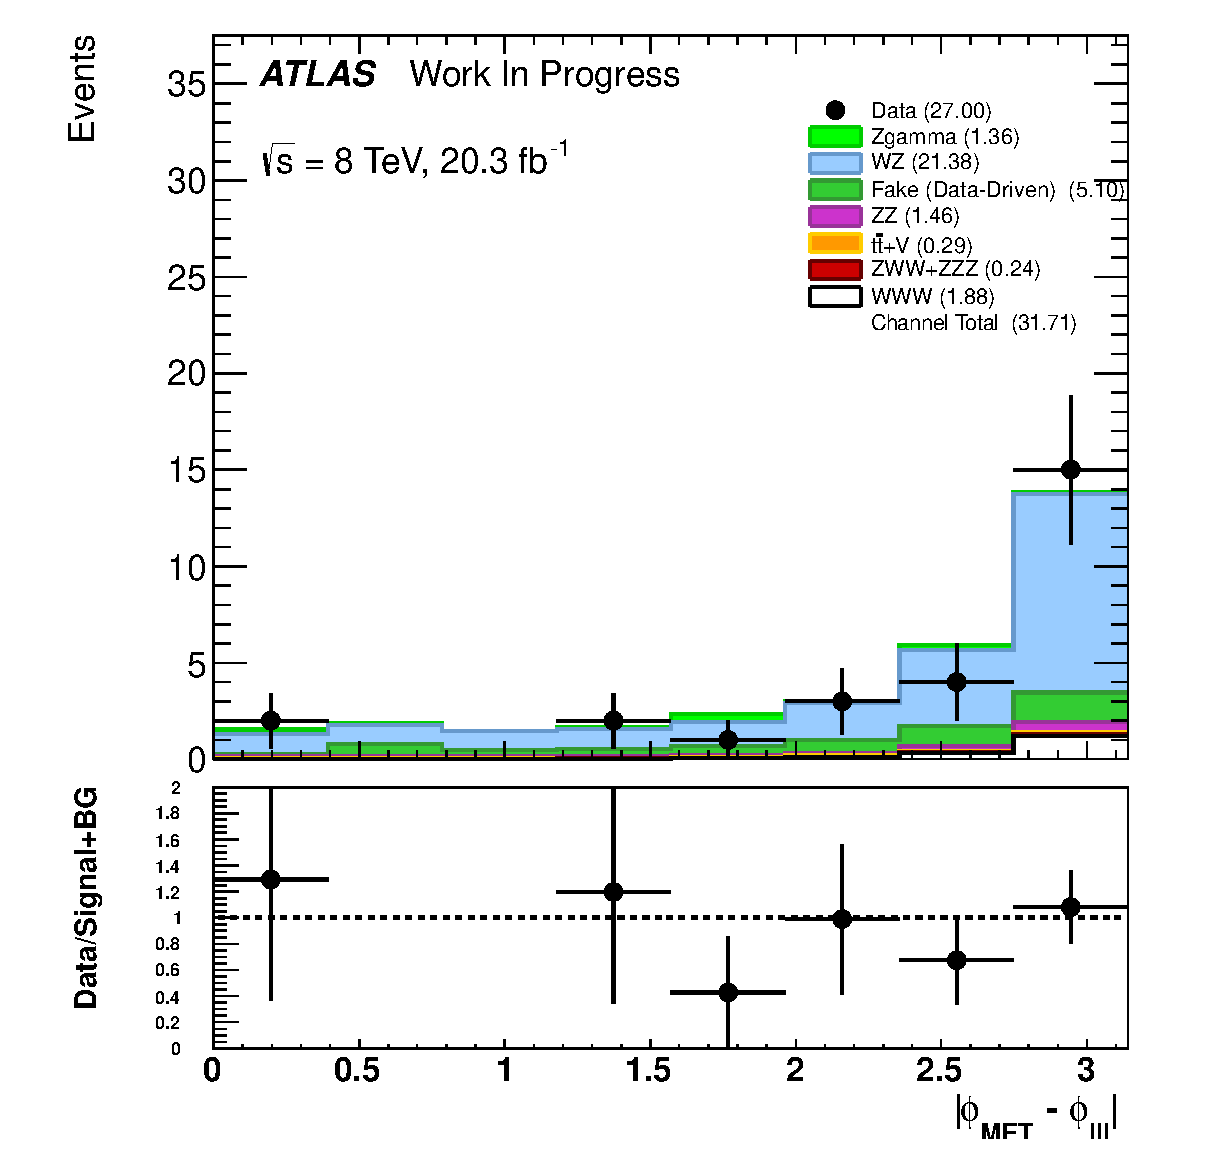
\includegraphics[width=0.3\columnwidth]{figures/appendix_signal_selection/PreselectionJune2_NoSTVF_1SFOS_ChargeAbs1_ZVetoLow35High25GeV_BVeto85_METGt45GeV_physics/weight_all/eps/DeltaPhiMET123_Abs_histratio.eps}
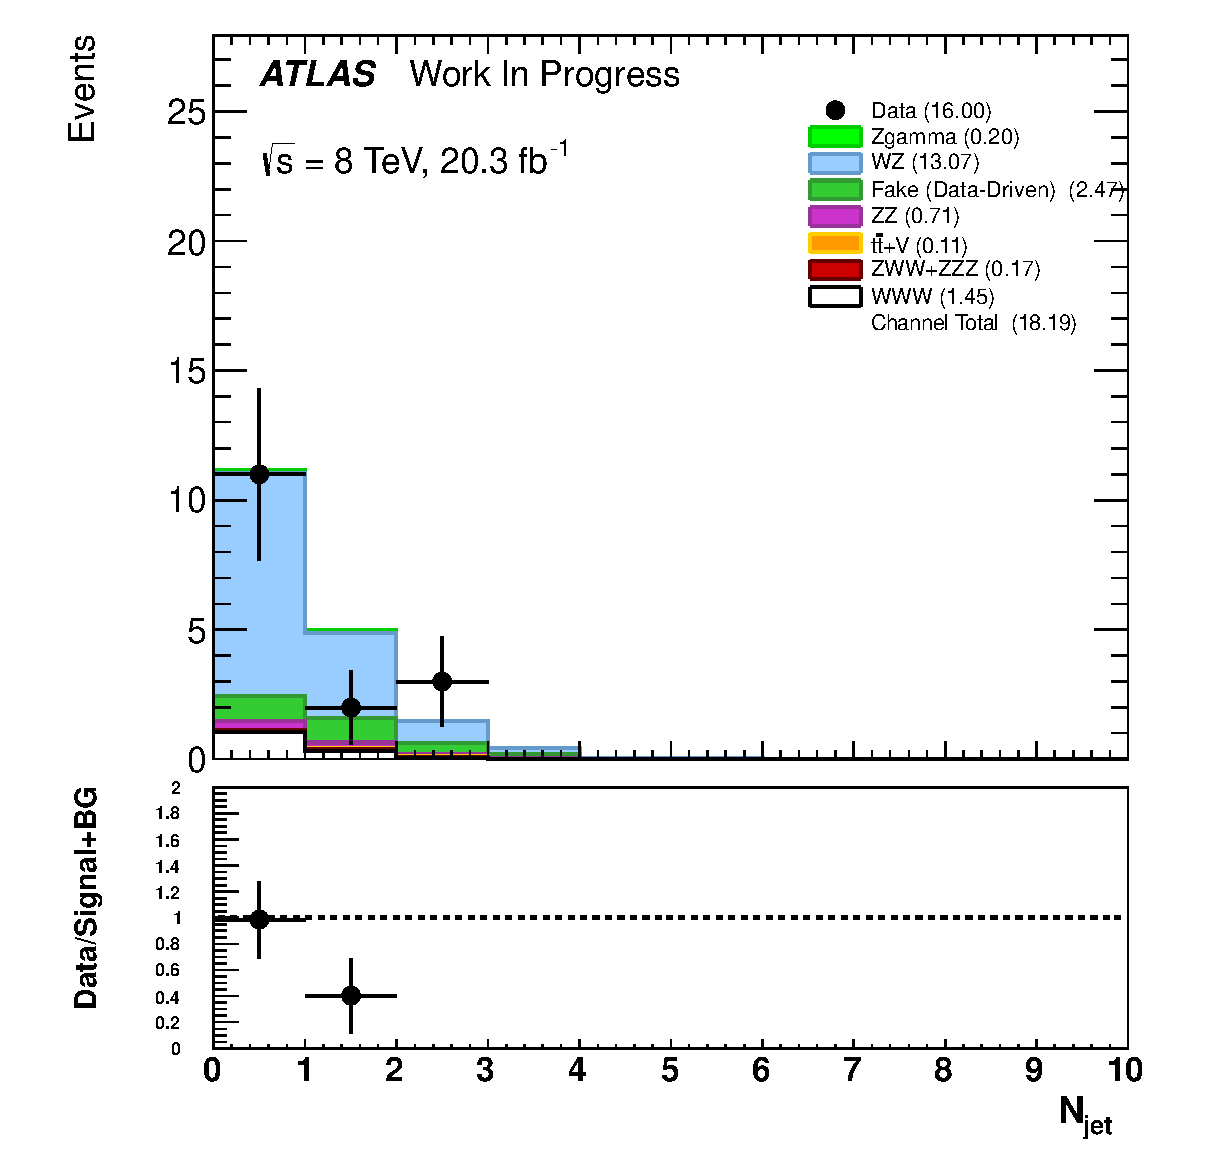
\includegraphics[width=0.3\columnwidth]{figures/appendix_signal_selection/PreselectionJune2_NoSTVF_1SFOS_ChargeAbs1_ZVetoLow35High25GeV_BVeto85_METGt45GeV_DeltaPhi2p5_physics/weight_all/eps/NJets_histratio.eps}
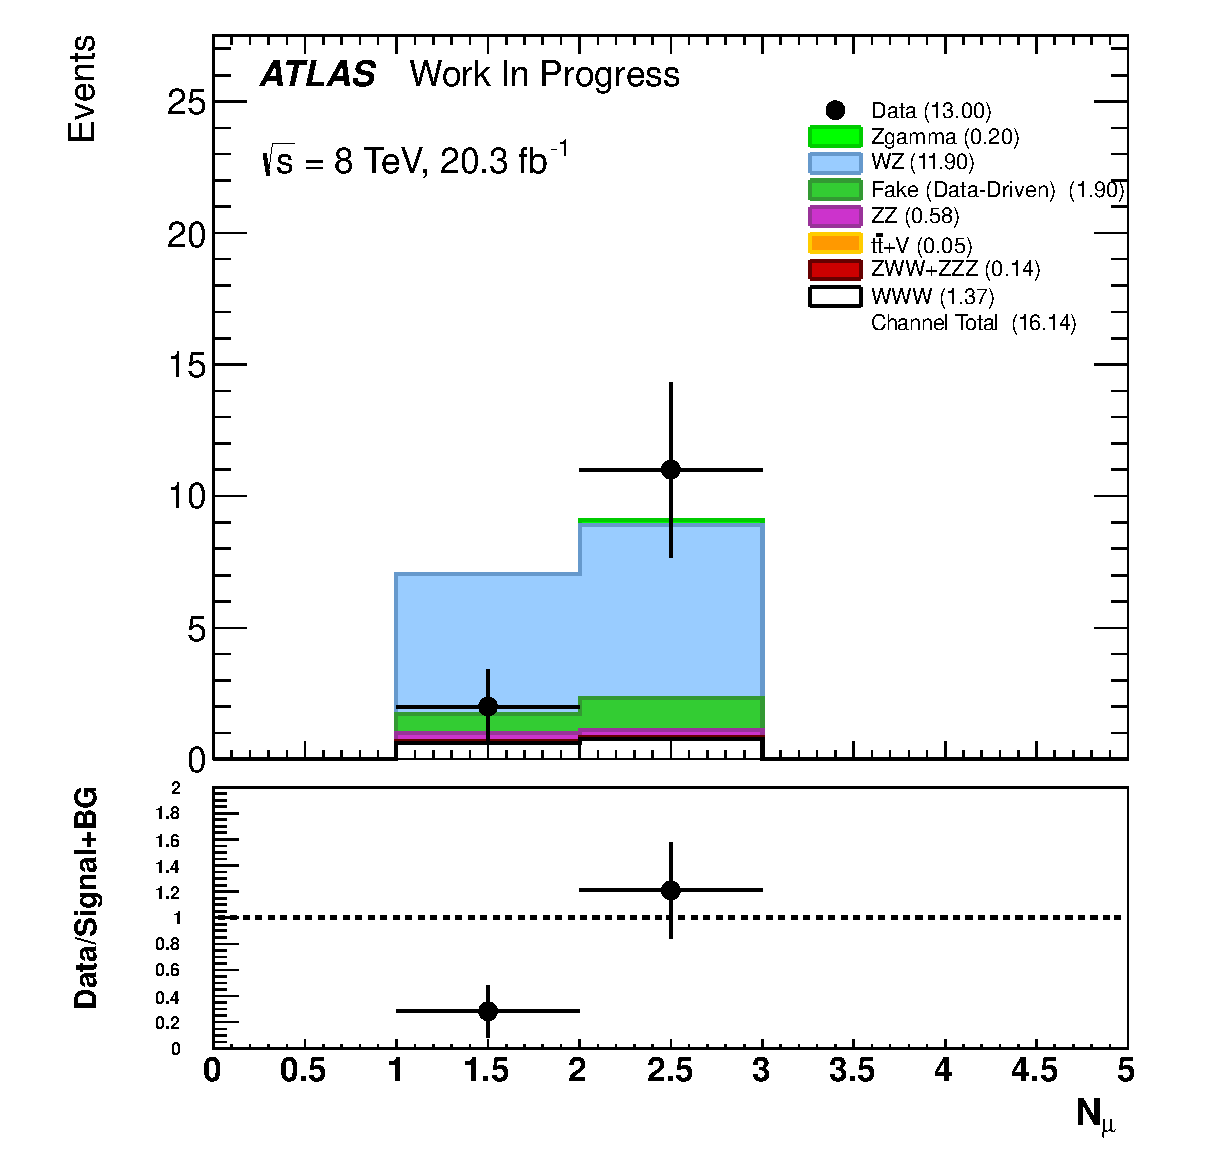
\includegraphics[width=0.3\columnwidth]{figures/appendix_signal_selection/PreselectionJune2_NoSTVF_1SFOS_ChargeAbs1_ZVetoLow35High25GeV_BVeto85_METGt45GeV_DeltaPhi2p5_NJetLt2_physics/weight_all/eps/NMuons_histratio.eps}
\caption{Distributions showing data compared to the signal plus background estimate in the 1 SFOS region at each stage 
of the selection before the cuts are applied to the given distribution. Plots should be read sequentially from left to right
and from top to bottom. 
Referring to Table~\ref{tab:cutflow_weighted_1sfos}, the top left
plot is shown before cut \#3 is applied, top middle is before cut \#4, and
so on until the bottom right which is after all cuts are applied.}
\label{fig:1sfos}
\end{figure}


%\begin{table}[ht!]
%\centering
%\begin{tabular}{|c||c|c|c|c|}
\hline
 & $eee$ & $ee\mu$ & $e\mu\mu$ & $\mu\mu\mu$\\ 
\hline\hline
$WZ$ &  $0.0 \pm 0$ &  $5.321 \pm 0.099$ &  $6.58 \pm 0.11$ &  $0.0 \pm 0$\\ 
$ZZ$ &  $0.0 \pm 0$ &  $0.324 \pm 0.012$ &  $0.259 \pm 0.011$ &  $0.0 \pm 0$\\ 
$Z\gamma$ &  $0.0 \pm 0$ &  $0.0 \pm 0$ &  $0.20 \pm 0.13$ &  $0.0 \pm 0$\\ 
$ZWW+ZZZ$ &  $0.0 \pm 0$ &  $0.0660 \pm 0.0077$ &  $0.074 \pm 0.008$ &  $0.0 \pm 0$\\ 
$t\bar{t}+V$ &  $0.0 \pm 0$ &  $0.0207 \pm 0.0031$ &  $0.0296 \pm 0.0036$ &  $0.0 \pm 0$\\ 
Fake (data-driven) &  $0.0 \pm 0$ &  $0.71 \pm 0.18$ &  $1.19 \pm 0.29$ &  $0.0 \pm 0$\\ 
$WWW$ &  $0.0 \pm 0$ &  $0.61 \pm 0.01$ &  $0.760 \pm 0.012$ &  $0.0 \pm 0$\\ 
\hline
Expected Background &  $0.0 \pm 0$ &  $6.44 \pm 0.21$ &  $8.33 \pm 0.34$ &  $0.0 \pm 0$\\ 
Expected Signal + Background &  $0.0 \pm 0$ &  $7.05 \pm 0.21$ &  $9.09 \pm 0.34$ &  $0.0 \pm 0$\\ 
\hline
Observed Data &  $0.0 \pm 0$ &  $2.0 \pm 1.4$ &  $11.0 \pm 3.3$ &  $0.0 \pm 0$\\ 
\hline
\end{tabular}

%\caption{ Expected and observed event yields binned by lepton flavor combination for the optimized 1 SFOS signal region selection defined as follows: event pre-selection + 1 SFOS + b-veto + Z-veto + $\Delta\phi$ + $N_{jet}$ requirements.
%Only statistical uncertainties are shown.
%}
%\label{tab:1sfos}
%\end{table}

\clearpage
\subsubsection{2 SFOS Signal Region}
The cutflows for the selection in the 2 SFOS region are shown in Table~\ref{tab:cutflow_weighted_2sfos}
while the distributions at each stage of the selection are shown in Figure~\ref{fig:2sfos}.
Even though, the expected background is lower in this region than in the 1 SFOS region, this is the least sensitive signal region 
due to a similar signal efficiency in this region as compared to the 1 SFOS region.
The signal to background ratio is 5.8\% with the dominant background being due to $WZ$, similar to the 1 SFOS region.
There is a fairly large discrepancy observed between the total prediction and the data in this region that is (possibly)
about 2-3 sigma if considering systematic uncertainties reported in Table~\ref{tab:sys_summary}.
The discrepancy is similar for both the $eee$ and $\mu\mu\mu$ lepton flavor combinations as can be seen in the bottom
right of Figure~\ref{fig:2sfos}. If we examine the other distributions of Figure~\ref{fig:2sfos} we see that
the discrepancy begins to appear at the cut on $E_{T}^{Miss} > 55$~GeV. The $E_{T}^{Miss}$ distribution is shown in the
top right of Figure~\ref{fig:2sfos} before the cut is applied. Here we can see that the prediction shows reasonably good
agreement with the data, with only 2 bins showing a discrepancy larger than 1 sigma from the statistical uncertainty. However,
after the cut on $E_{T}^{Miss}$, one of these discrepant bins ends up being the highest contribution to the overall estimate, thus
enhancing the disagreement. This suggests that the disagreement may just be due to a statitical fluctuation.
The poisson probability of observing 6 events with 10.86 events expected from the signal plus background prediction is 5.7\%.

\begin{table}[ht!]
\centering
\scriptsize
\begin{tabular}{l||c|c||c|c||c|c||c|c||c|c||c|c||c|c||c|c}
\hline
 &                 \multicolumn{2}{c||}{Signal}            &  \multicolumn{12}{c||}{Background} &  \multicolumn{2}{c}{Data} \\
 & &  & \multicolumn{2}{c||}{$WZ$} & \multicolumn{2}{c||}{$ZZ$} & \multicolumn{2}{c||}{$t\bar{t}+V$} & \multicolumn{2}{c||}{$ZZZ+ZWW$} & \multicolumn{2}{c||}{$Z\gamma$} & \multicolumn{2}{c||}{Fake} &  & \\ 
 & Yield & Eff. & Yield & Eff. & Yield & Eff. & Yield & Eff. & Yield & Eff. & Yield & Eff. & Yield & Eff.  & Yield & Eff.\\
\hline\hline
1. Pre-selection &  $9.61$ & --- &  $1566.91$ & --- &  $323.60$ & --- &  $36.93$ & --- &  $3.12$ & --- &  $219.80$ & --- &  $238.12$ & ---  & $2472$ &  --- \\ 
\hline
2. 2 SFOS &  $2.61$ &  $0.27$ &  $807.27$ &  $0.52$ &  $151.28$ &  $0.47$ &  $15.35$ &  $0.42$ &  $1.30$ &  $0.41$ &  $69.99$ &  $0.32$ &  $87.34$ &  $0.37$ & $1182$ &  $0.48$\\ 
\hline
3. $N_{\mathrm{b-jet}}=0$ &  $2.46$ &  $0.94$ &  $743.12$ &  $0.92$ &  $136.16$ &  $0.90$ &  $1.19$ &  $0.08$ &  $1.10$ &  $0.85$ &  $64.70$ &  $0.92$ &  $65.80$ &  $0.75$ & $1033$ &  $0.87$\\ 
\hline
4. $| m_{\mathrm{SFOS}} - m_Z | >  20$ GeV &  $1.43$ &  $0.58$ &  $44.95$ &  $0.06$ &  $21.13$ &  $0.16$ &  $0.22$ &  $0.18$ &  $0.19$ &  $0.17$ &  $29.52$ &  $0.46$ &  $12.87$ &  $0.20$ & $108$ &  $0.10$\\ 
\hline
5. $E_{T}^{Miss} > 55$ GeV &  $0.82$ &  $0.57$ &  $15.86$ &  $0.35$ &  $0.97$ &  $0.05$ &  $0.14$ &  $0.65$ &  $0.12$ &  $0.63$ &  $0.43$ &  $0.01$ &  $1.47$ &  $0.11$ & $18$ &  $0.17$\\ 
\hline
6. $|\Delta\phi(3l,E_{T}^{Miss})| > 2.5$ &  $0.64$ &  $0.78$ &  $10.09$ &  $0.64$ &  $0.55$ &  $0.57$ &  $0.07$ &  $0.49$ &  $0.10$ &  $0.82$ &  $0.11$ &  $0.25$ &  $0.72$ &  $0.49$ & $8$ &  $0.44$\\ 
\hline
7. $N_{\mathrm{Jet}} \leq 1$ &  $0.60$ &  $0.94$ &  $9.07$ &  $0.90$ &  $0.48$ &  $0.86$ &  $0.02$ &  $0.35$ &  $0.08$ &  $0.82$ &  $0.11$ &  $1.00$ &  $0.49$ &  $0.69$ & $6$ &  $0.75$\\ 
\hline
\end{tabular}


\caption{Cutflows showing the event yields and efficiencies for each cut in the 2 SFOS signal region
starting from event pre-selection and binned by category. 
Event yields for MC backgrounds and signal include all weights and are normalized to an integrated luminosity of $20.3~\mathrm{fb}^{-1}$.  
The fake lepton background only includes the matrix method weights.  The data is unweighted.
Efficiencies show the ratio of the yield with respect
to the previous cut.  The efficiency is first calculated at the first cut after event pre-selection.  }
\label{tab:cutflow_weighted_2sfos}
\end{table}


%2 SFOS consolidated
\begin{figure}[ht!]
\centering
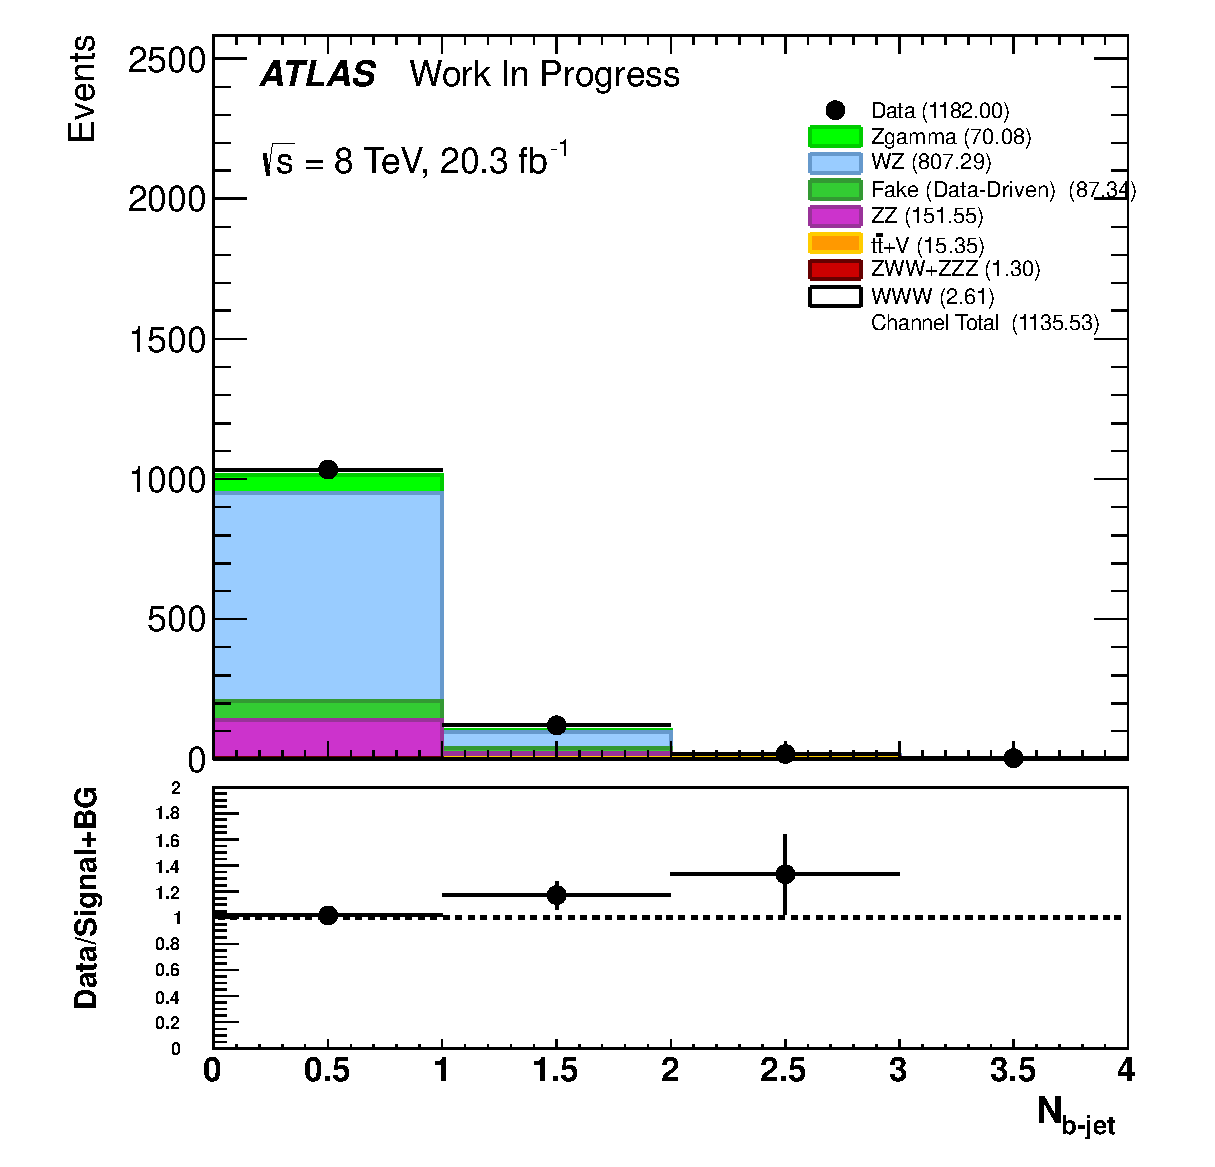
\includegraphics[width=0.3\columnwidth]{figures/appendix_signal_selection/PreselectionMay29_2SFOS_ChargeAbs1_physics/weight_all/eps/NBTaggedJets_histratio.eps}
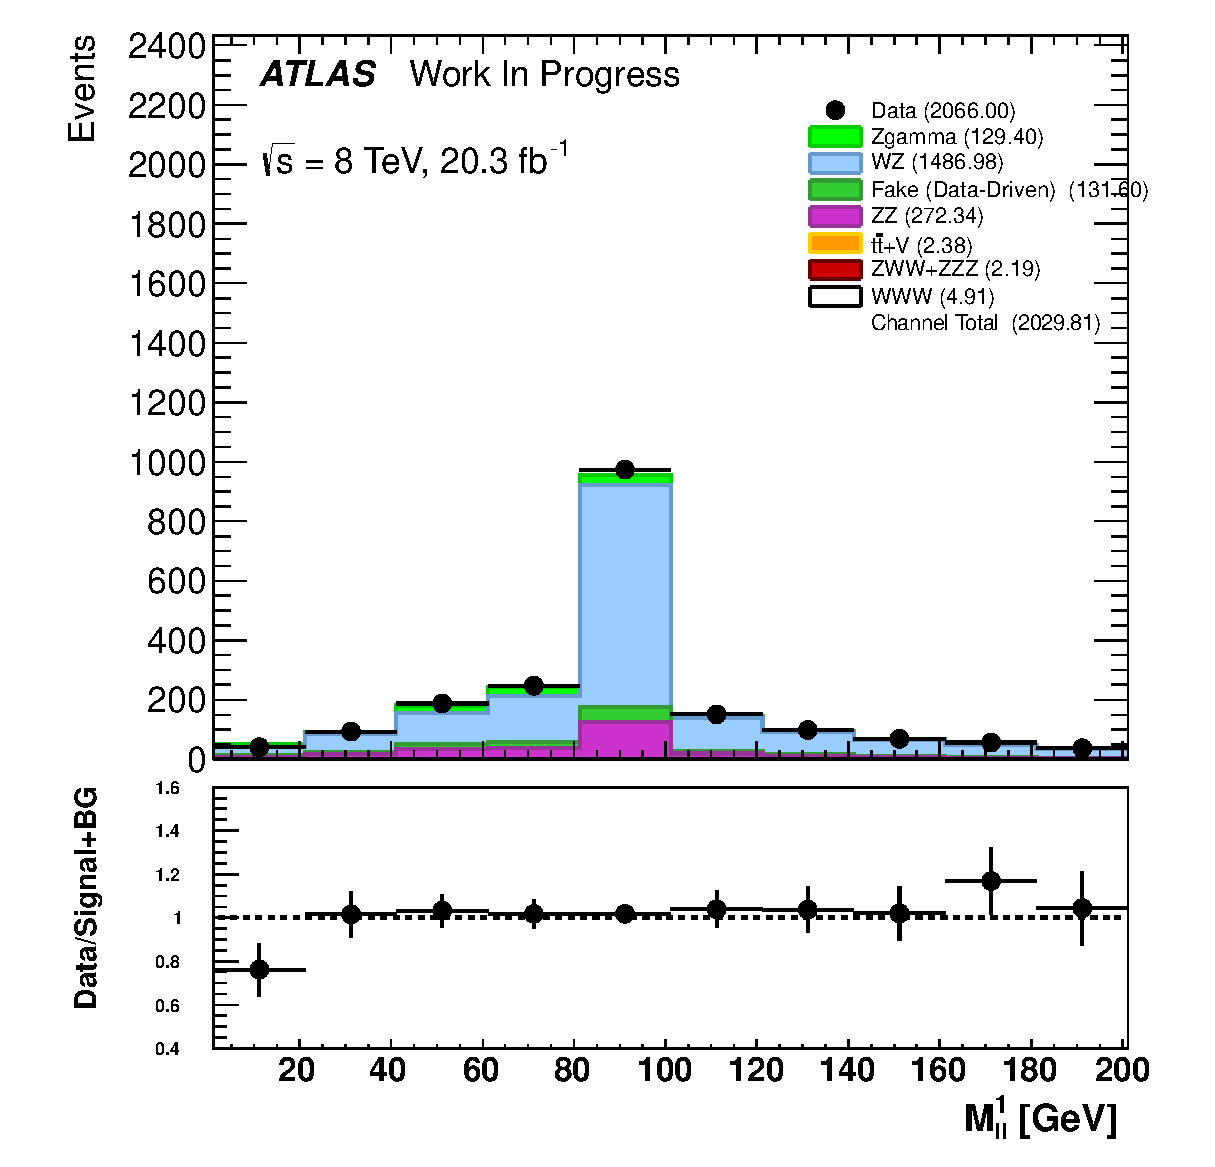
\includegraphics[width=0.3\columnwidth]{figures/appendix_signal_selection/PreselectionMay29_2SFOS_ChargeAbs1_BVeto85_physics/weight_all/eps/InvariantMassSFOS_histratio.eps}
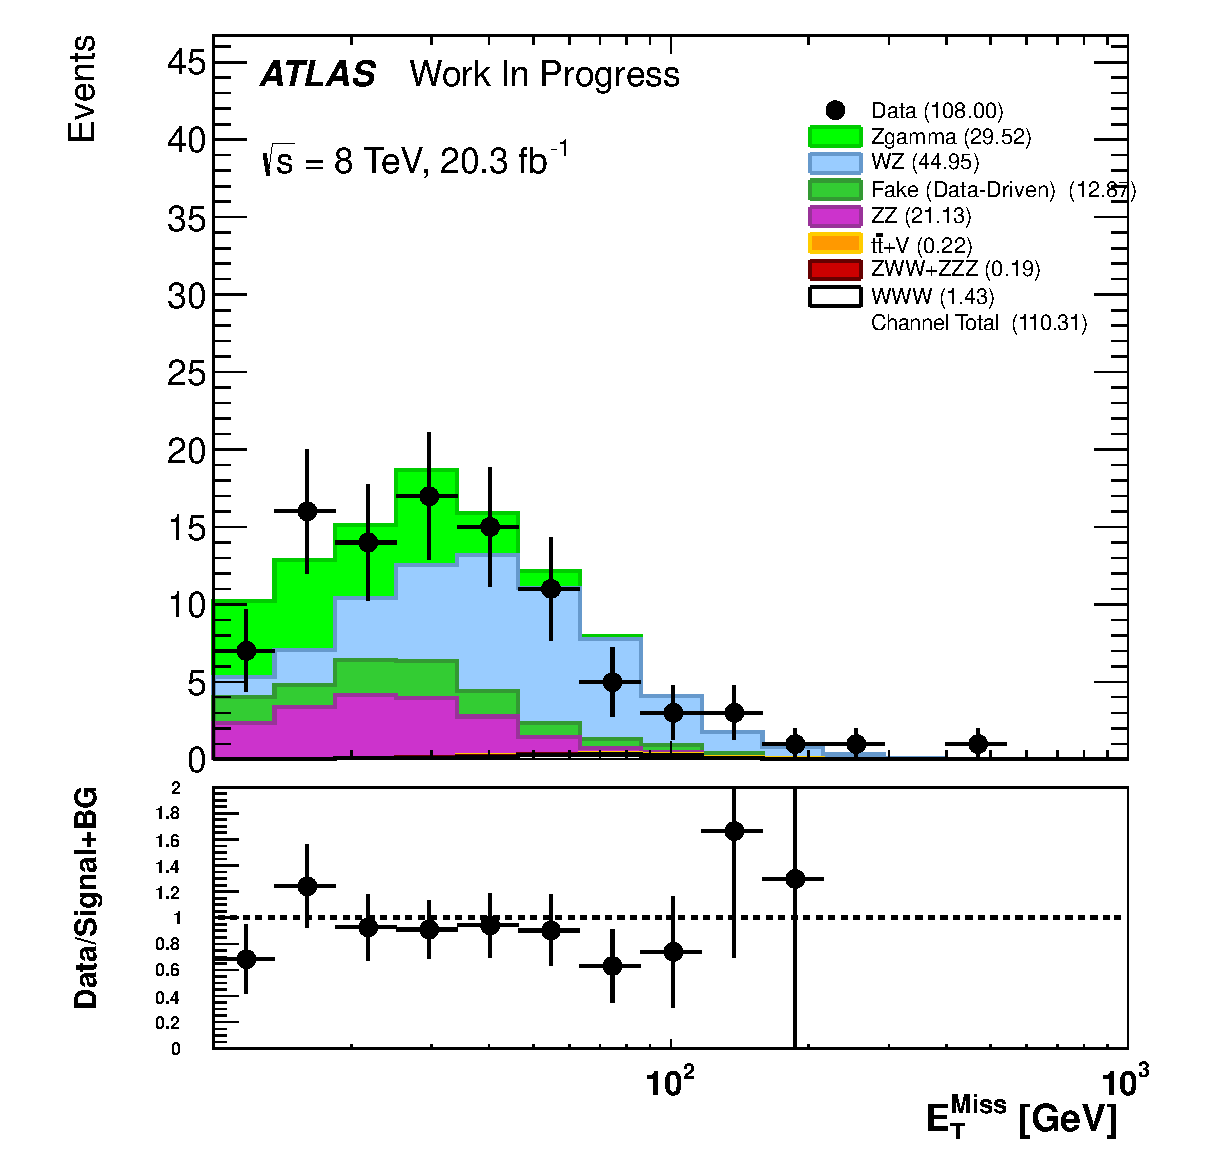
\includegraphics[width=0.3\columnwidth]{figures/appendix_signal_selection/PreselectionMay29_2SFOS_ChargeAbs1_BVeto85_ZVeto20GeV_physics/weight_all/eps/MET_Et_histratio.eps}
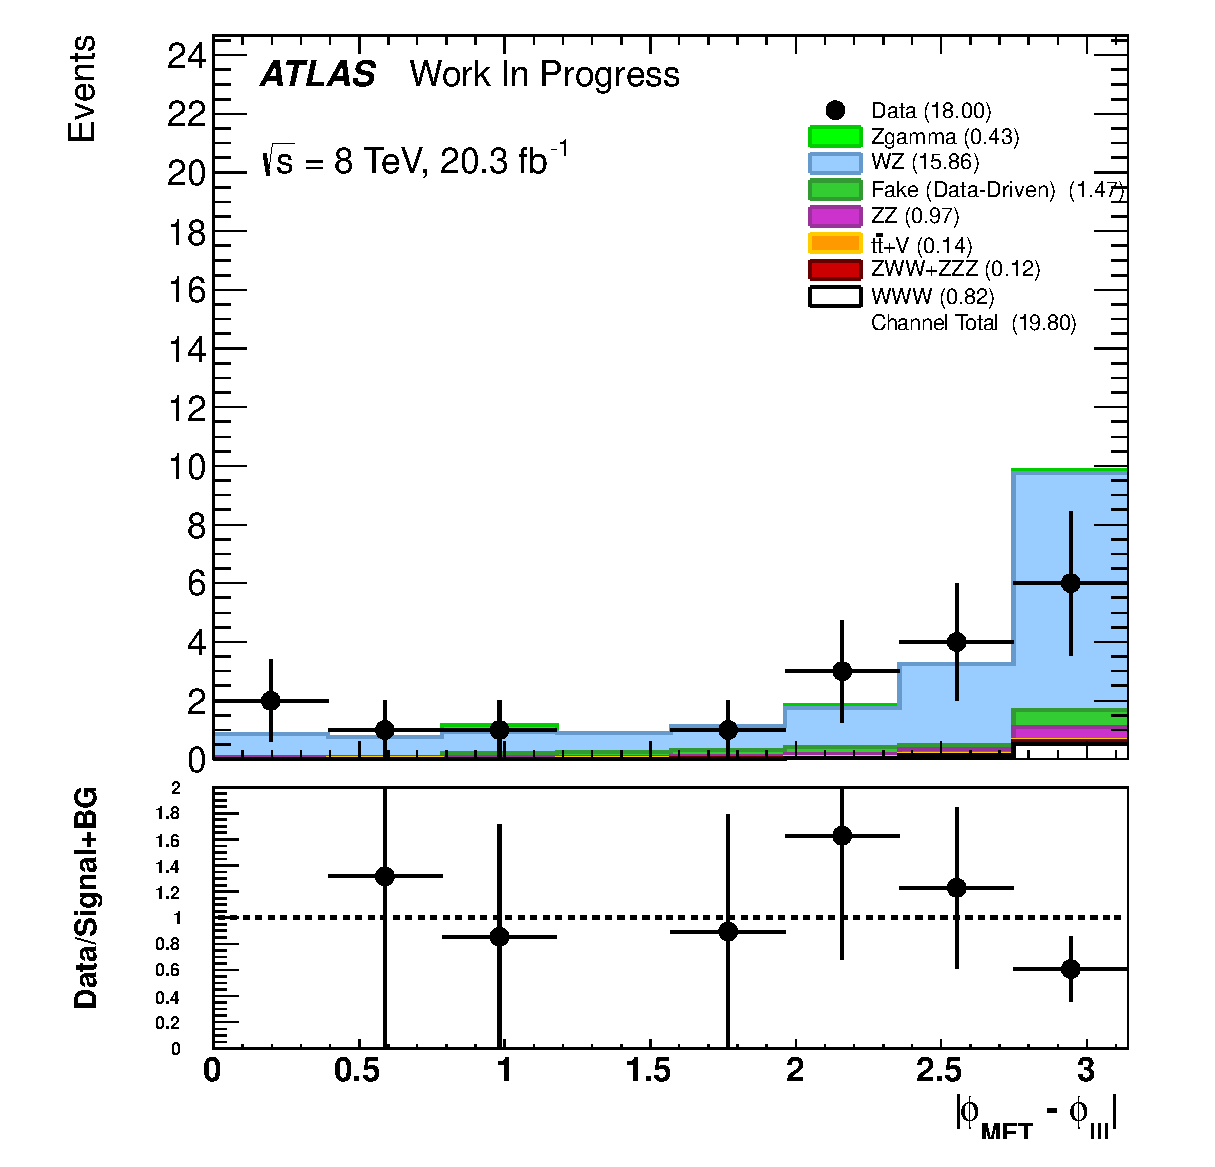
\includegraphics[width=0.3\columnwidth]{figures/appendix_signal_selection/PreselectionJune2_NoSTVF_2SFOS_ChargeAbs1_BVeto85_ZVeto20GeV_METGt55GeV_physics/weight_all/eps/DeltaPhiMET123_Abs_histratio.eps}
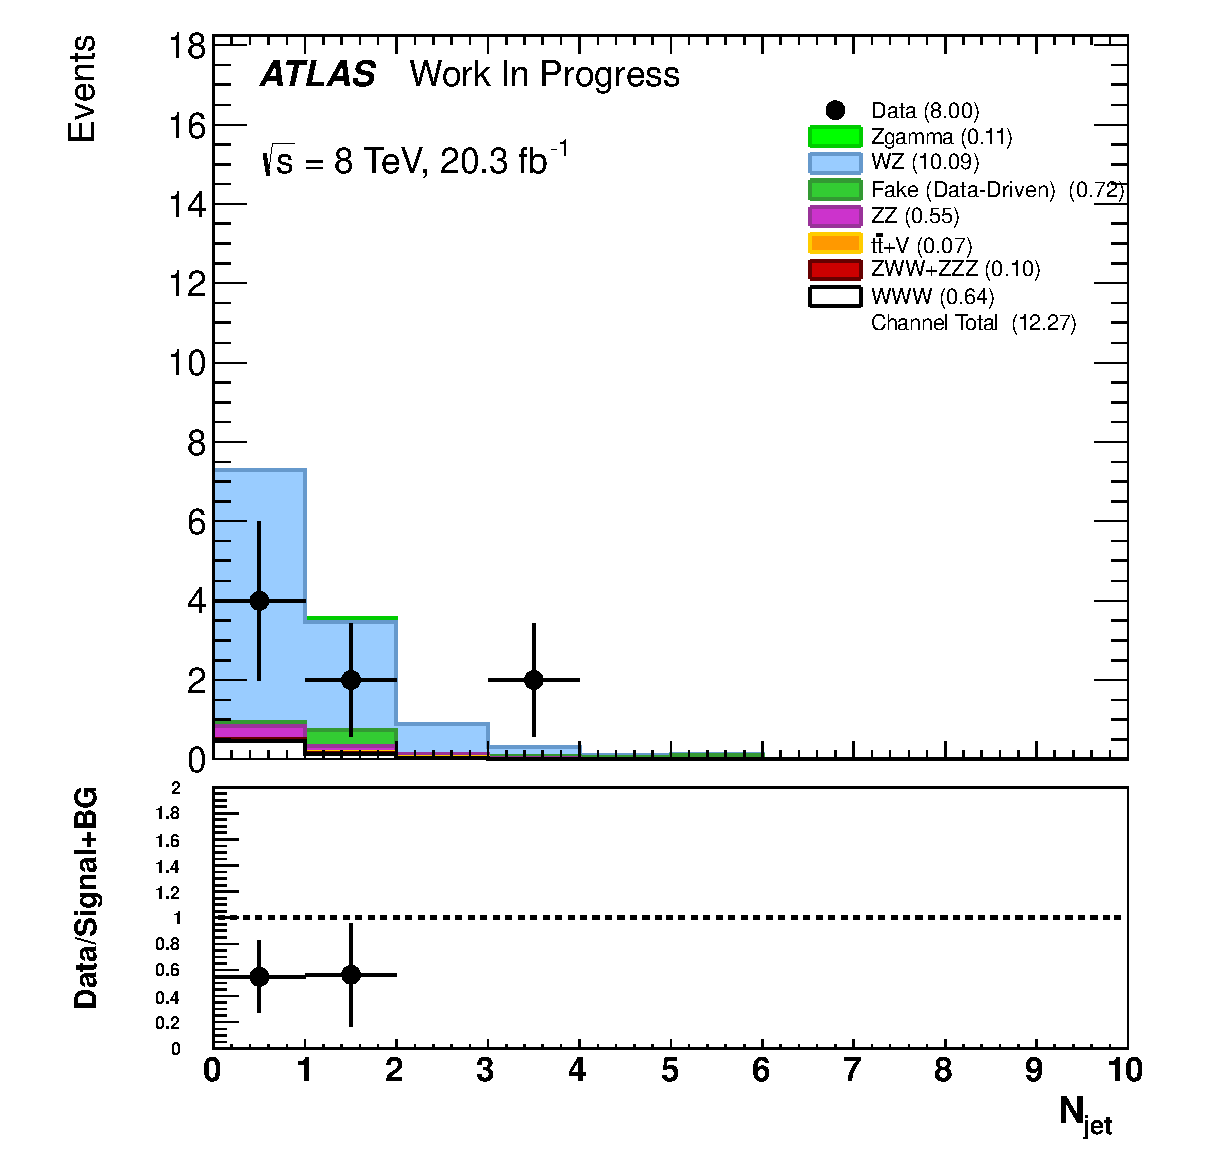
\includegraphics[width=0.3\columnwidth]{figures/appendix_signal_selection/PreselectionJune2_NoSTVF_2SFOS_ChargeAbs1_BVeto85_ZVeto20GeV_METGt55GeV_DeltaPhi2p5_physics/weight_all/eps/NJets_histratio.eps}
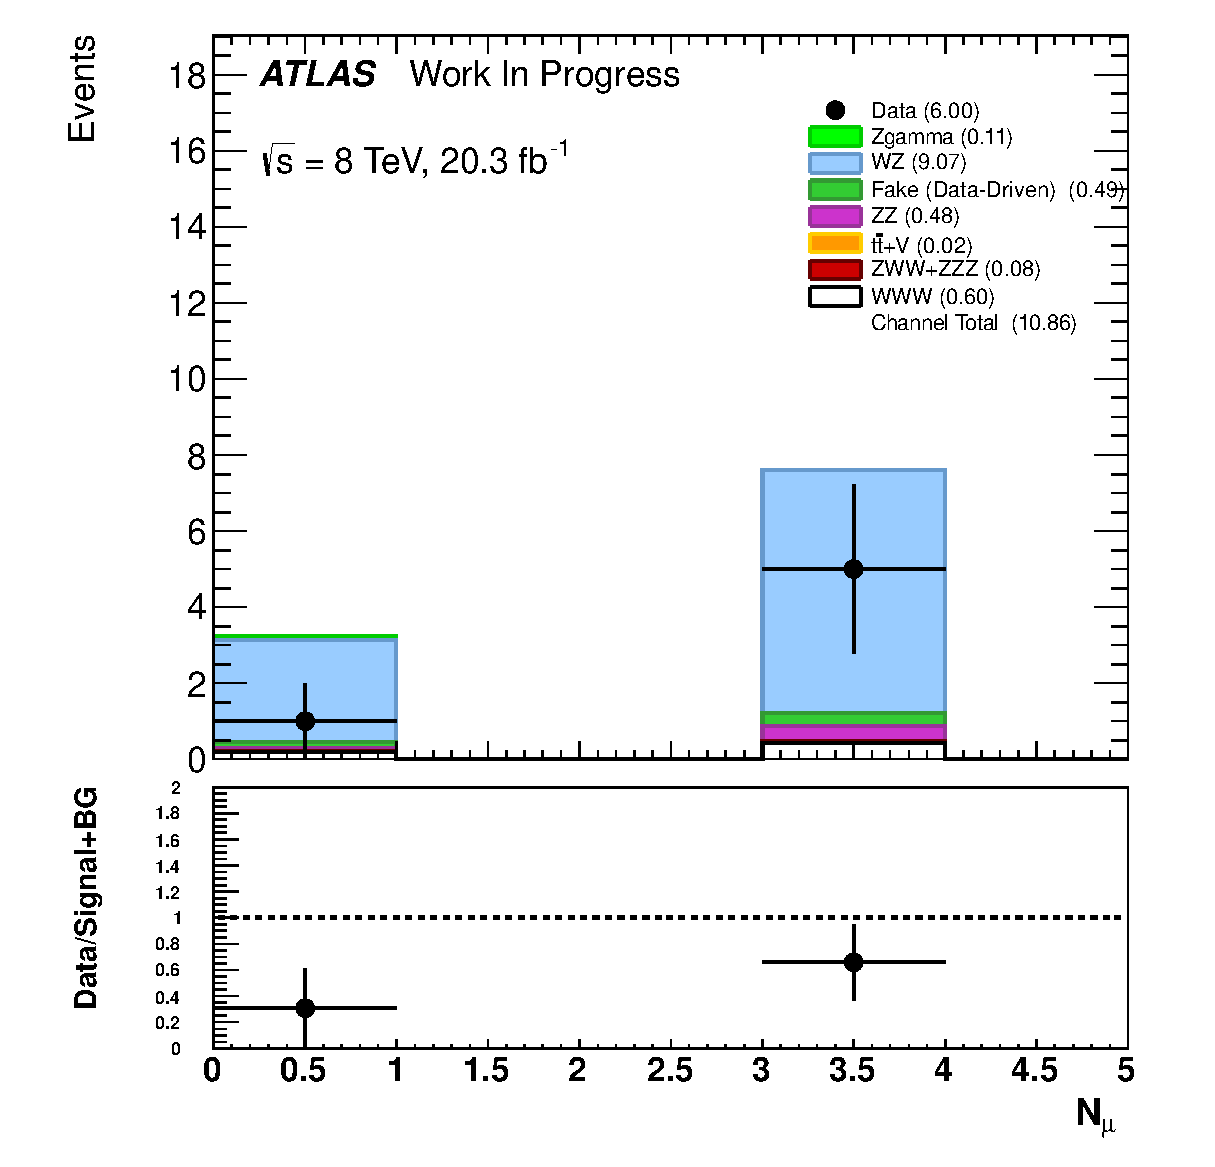
\includegraphics[width=0.3\columnwidth]{figures/appendix_signal_selection/PreselectionJune2_NoSTVF_2SFOS_ChargeAbs1_BVeto85_ZVeto20GeV_METGt55GeV_DeltaPhi2p5_NJetLt2_physics/weight_all/eps/NMuons_histratio.eps}
\caption{Distributions showing data compared to the signal plus background estimate in the 2 SFOS region at each stage 
of the selection before the cuts are applied to the given distribution. Plots should be read sequentially from left to right
and from top to bottom. 
Referring to Table~\ref{tab:cutflow_weighted_2sfos}, the top left
plot is shown before cut \#3 is applied, the top middle is before cut \#4, and
so on until the bottom right which is after all cuts are applied.}
\label{fig:2sfos}
\end{figure}



%\begin{table}[ht!]
%\centering
%\begin{tabular}{|c||c|c|c|c|}
\hline
 & $eee$ & $ee\mu$ & $e\mu\mu$ & $\mu\mu\mu$\\ 
\hline\hline
$WZ$ &  $2.69 \pm 0.07$ &  $0.0 \pm 0$ &  $0.0 \pm 0$ &  $6.39 \pm 0.11$\\ 
$ZZ$ &  $0.0800 \pm 0.0046$ &  $0.0 \pm 0$ &  $0.0 \pm 0$ &  $0.3970 \pm 0.0098$\\ 
$Z\gamma$ &  $0.110 \pm 0.096$ &  $0.0 \pm 0$ &  $0.0 \pm 0$ &  $0.0 \pm 0$\\ 
$ZWW+ZZZ$ &  $0.0292 \pm 0.0046$ &  $0.0 \pm 0$ &  $0.0 \pm 0$ &  $0.0493 \pm 0.0066$\\ 
$t\bar{t}+V$ &  $0.0063 \pm 0.0016$ &  $0.0 \pm 0$ &  $0.0 \pm 0$ &  $0.0176 \pm 0.0029$\\ 
Fake (data-driven) &  $0.16 \pm 0.12$ &  $0.0 \pm 0$ &  $0.0 \pm 0$ &  $0.3 \pm 0.1$\\ 
$WWW$ &  $0.1819 \pm 0.0055$ &  $0.0 \pm 0$ &  $0.0 \pm 0$ &  $0.4212 \pm 0.0086$\\ 
\hline
Expected Background &  $3.07 \pm 0.17$ &  $0.0 \pm 0$ &  $0.0 \pm 0$ &  $7.19 \pm 0.15$\\ 
Expected Signal + Background &  $3.25 \pm 0.17$ &  $0.0 \pm 0$ &  $0.0 \pm 0$ &  $7.61 \pm 0.15$\\ 
\hline
Observed Data &  $1.0 \pm 1$ &  $0.0 \pm 0$ &  $0.0 \pm 0$ &  $5.0 \pm 2.2$\\ 
\hline
\end{tabular}

%\caption{ Expected and observed event yields binned by lepton flavor combination for the optimized 2 SFOS signal region selection defined as follows: event pre-selection + 2 SFOS + b-veto + Z-veto + $\Delta\phi$ + $N_{jet}$ requirements.
%Only statistical uncertainties are shown.
%}
%\label{tab:2sfos}
%\end{table}

\subsubsection{Signal Efficiency }
\label{sec:signal_efficiency}

The signal efficiency, $\varepsilon_i$, is defined for each channel, $i$,
as the ratio of the number of expected signal events measured
at the reconstruction level, $N_i^{\textrm{Signal}}$, over the fiducial cross-section, $\sigma^{\textrm{Fiducial}}_i$, times the integrated luminosity:
\begin{equation}
\varepsilon_i = \frac{N_i^{\textrm{Signal}}}{\sigma^{\textrm{Fiducial}}_i\cdot\int\mathscr{L}~\textrm{d}t}
\end{equation}
Recall that the fiducial cross-sections are presented in Section~\ref{sec:fiducial_cross_section}. Further, the fiducial cross-section definition
does not include the branching fraction from $W\rightarrow\tau\nu$ decays.
We observe by looking at truth information that about 20\% of signal
events reconstructed at truth level contain at
least one $W\rightarrow\tau\nu$ decay. Thus, the signal efficiency
definition includes this level of contamination from these events
even though they do not belong explicitly to our signal definition.
Using the reconstructed signal yields listed above and the fiducial
cross-sections generated using MadGraph
from Table~\ref{tab:fiducial_cross_sections}, we
arrive at the signal efficiencies listed in Table~\ref{tab:signal_efficiencies}.


\begin{table}[ht!]
\centering
\begin{tabular}{|c||c|}
\hline
Channel & Signal Efficiency \\
\hline\hline
0 SFOS &  $0.567 \pm .022$ \\
1 SFOS &  $0.533 \pm .019$ \\
2 SFOS &  $0.589 \pm .033$ \\
\hline
\end{tabular}

\caption{Signal efficiencies derived separately for each signal region. Only statistical uncertainties are shown.}
\label{tab:signal_efficiencies}
\end{table}




